\section{Model training and evaluation}\label{Model training and evaluation}

This section presents an overview of the primary guiding principals used during the stages of model training and evaluation.

\subsection{Bias-Variance dilemma}\label{Bias-Variance dilemma}

The bias-variance dilemma is a fundamental problem in machine learning and involves the issues of model optimization and generalization. In the case of optimization (reducing the model error) a model eventually starts to overfit the training data, this results in high error of the models predictions on the test/validation datasets (high variance). The opposite is aiming to increase model generalization (reduction of model complexity) however this in turn causes underfitting or high error of the models predictions on the training dataset (high bias). This counterpoised behaviour of both bias and variance enables the easy assessment of model suitability for use in the prediction of unseen data \cite{ibm-ensemble,ibm-regularization,svm-2}.

% Juxtaposed
%
% In the case of generalization (reduction of model complexity) a model starts to underfit the training data, this results in high error of the models predictions on the training dataset (high bias).
%
% The opposite is aiming to increase model optimization (reducing the model error) however this in turn pushed to far causes overfitting or high error of the models predictions on the test/validation datasets (high variance).

\subsection{Performance metric}\label{Performance metric}

The accuracy of the model forecasts was evaluated on the basis of the \glsxtrlong{mse} this metric measures the average squared difference between predicted and actual values, providing a sense of the magnitude of the errors. A lower \gls{mse} indicates better fit, but it is sensitive to outliers due to the squaring of errors \cite{scikit-mse}.

$$MSE = \frac{1}{n} \sum_{i=1}^{n} (y_i - \hat{y}_i)^2$$

Where:
\begin{itemize}
    \item $n$ is the total number of predictions
    \item $y_i$ is the actual value at time $i$
    \item $\hat{y}_i$ is the predicted value at time $i$
\end{itemize}

\subsection{Methodology}\label{Methodology}

The process of model training and evaluation consisted of model fitting using the Optuna hyperparameter optimization framework with the goal of minimizing the \gls{mse} followed by data analysis of the obtained optized forecasts. During analysis for each model accuracy was evaluated on both in-sample (training set) and out-of-sample (test set) data. The preprocessing variant yielding the minimum average \gls{mse} across all offsets (train and test sets combined) was selected as optimal.

\subsubsection{Optuna model fitting}\label{Optuna model fitting}

In the first step each of the models was fitted on different suitable dataset processing variations. For the purpose of efficient and reproducible hyperparameter optimization that exceeds what can be achieved within reasonable time frames using the GridSearchCV class from scikit-learn, an alternative drop-in replacement class OptunaSearchCV provided by the Optuna package was used instead. Unlike grid search's exhaustive enumeration, Optuna's \gls{tpe} sampler efficiently explores the hyperparameter space through Bayesian optimization, focusing computational effort on promising regions of the hyperparameter space. For the \gls{mlp} only datasets for which normalization was applied as the last step were used. For the \gls{rf} all dataset processing variations were evaluated. For \gls{svr} only datasets processing methods that ended with standardization were used.

Beyond the parameters being optimized each model was used with its default parameters with some exceptions. For the \gls{mlp} the activation function was changed to \gls{tanh} due to the normalization range of the data, shuffle was set to false to prevent data shuffling in order to not disrupt the continuous time series nature of the data, random state was set to zero for reproducability of the results and the maximum number of iterations was increased to 10000 in order to allow for model convergence. For the \gls{rf} only the random state was set. For the \gls{svr} non of the default parameters were changed.

The parameters being optimized via OptunaSearchCV for each model as well as their selected value distributions are presented in table \ref{tab:mlp-hyperparams} for \gls{mlp}, table \ref{tab:rf-hyperparams} for \gls{rf}, table \ref{tab:svr-hyperparams} for \gls{svr} and table \ref{tab:arima-hyperparams} for \gls{arima}. The variable ranges were selected through manual experimentation to be broad and provide an ample search space for optimization.

OptunaSearchCV was run for 1000 iterations for each model for each applicable dataset variation for each offset from 1 to 12 months. All parameters were retained at default values other than 'scoring' which was set to 'neg\_mean\_squared\_error'.

\begin{table}[h]
    \centering
    \caption{Optuna hyperparameter search space for MLPRegressor}
    \begin{tabular}{|c|c|}
        \hline
        Parameter & Distribution \\
        \hline
        \hline
        hidden\_layer\_sizes & $Int(1, 30)$ \\
        \hline
        alpha & $Float(10^{-10}, 10^{-1})$ \\
        \hline
        tol & $Float(10^{-8}, 10^{-1})$ \\
        \hline
    \end{tabular}
    \label{tab:mlp-hyperparams}
\end{table}

\begin{table}[h]
    \centering
    \caption{Optuna hyperparameter search space for RandomForestRegressor}
    \begin{tabular}{|c|c|}
        \hline
        Parameter & Distribution \\
        \hline
        \hline
        n\_estimators & $Int(1, 40)$ \\
        \hline
        max\_depth & $Int(1, 40)$ \\
        \hline
        max\_features & $Int(1, 44)$ \\
        \hline
    \end{tabular}
    \label{tab:rf-hyperparams}
\end{table}

\begin{table}[h]
    \centering
    \caption{Optuna hyperparameter search space for SVR}
    \begin{tabular}{|c|c|}
        \hline
        Parameter & Distribution \\
        \hline
        \hline
        tol & $Float(10^{-6}, 10^{-1})$ \\
        \hline
        C & $Int(100, 2000)$ \\
        \hline
        $\epsilon$ & $Float(10^{-8}, 10^{-1})$ \\
        \hline
    \end{tabular}
    \label{tab:svr-hyperparams}
\end{table}

\begin{table}[h]
    \centering
    \caption{Optuna hyperparameter search space for ARIMA}
    \begin{tabular}{|c|c|}
        \hline
        Parameter & Distribution \\
        \hline
        \hline
        p & $Int(0, 6)$ \\
        \hline
        d & $Int(0, 6)$ \\
        \hline
        q & $Int(0, 6)$ \\
        \hline
    \end{tabular}
    \label{tab:arima-hyperparams}
\end{table}

\subsubsection{Data analysis}\label{Data analysis}

The forecasts obtained in the previous step were reverse transformed to obtain values in the same range as those of the original \gls{eer}. This was done due to the scale dependant nature of the \gls{mse} metric. Next for each dataset variation the cumulative averages for all offsets of the average \gls{mse} for both the training and test set forecasts were calculated.

% Step not intended for:
% - Comparing the MSE vs Hitrate not viable
% - Comparing models not viable

% Step intended for:
% - Comparing the results for various dataset preprocessing steps for each model in order to find best dataset processing variant
% - Basic trend observation

% General notes:
% - Models were optimized by MSE not Hitrate
% - Possible trends for description: best to worst

% Observations by case:
% - \gls{arima} \gls{mse}
%     + Best ld
%     + Worst ld that had been additionally scaled either via standardization of normalization.
%     + The best variation had a significantly smaller error than any other dataset variation
%     + The worst two ldn and lds had a significantly greater error than the rest of the dataset processing variations
%
% - \gls{arima} \gls{ds}
%     + The difference in \gls{ds} between the various dataset varients was not significant
% - \gls{mlp} \gls{mse}
% - \gls{mlp} \gls{ds}
% - \gls{rf} \gls{mse}
% - \gls{rf} \gls{ds}
% - \gls{svr} \gls{mse}
% - \gls{svr} \gls{ds}


As a result multiple rankings were obtained which can be seen in figure \ref{fig:mlp-mse} for \gls{mlp}, figure \ref{fig:rf-mse} for \gls{rf}, figure \ref{fig:svr-mse} for \gls{svr} and figure \ref{fig:arima-mse} for \gls{arima}. For the \gls{rw} model only the raw data was used.

% Bar charts for the average MSE and Hitrate for different dataset variations for each model

\begin{figure}[h]
    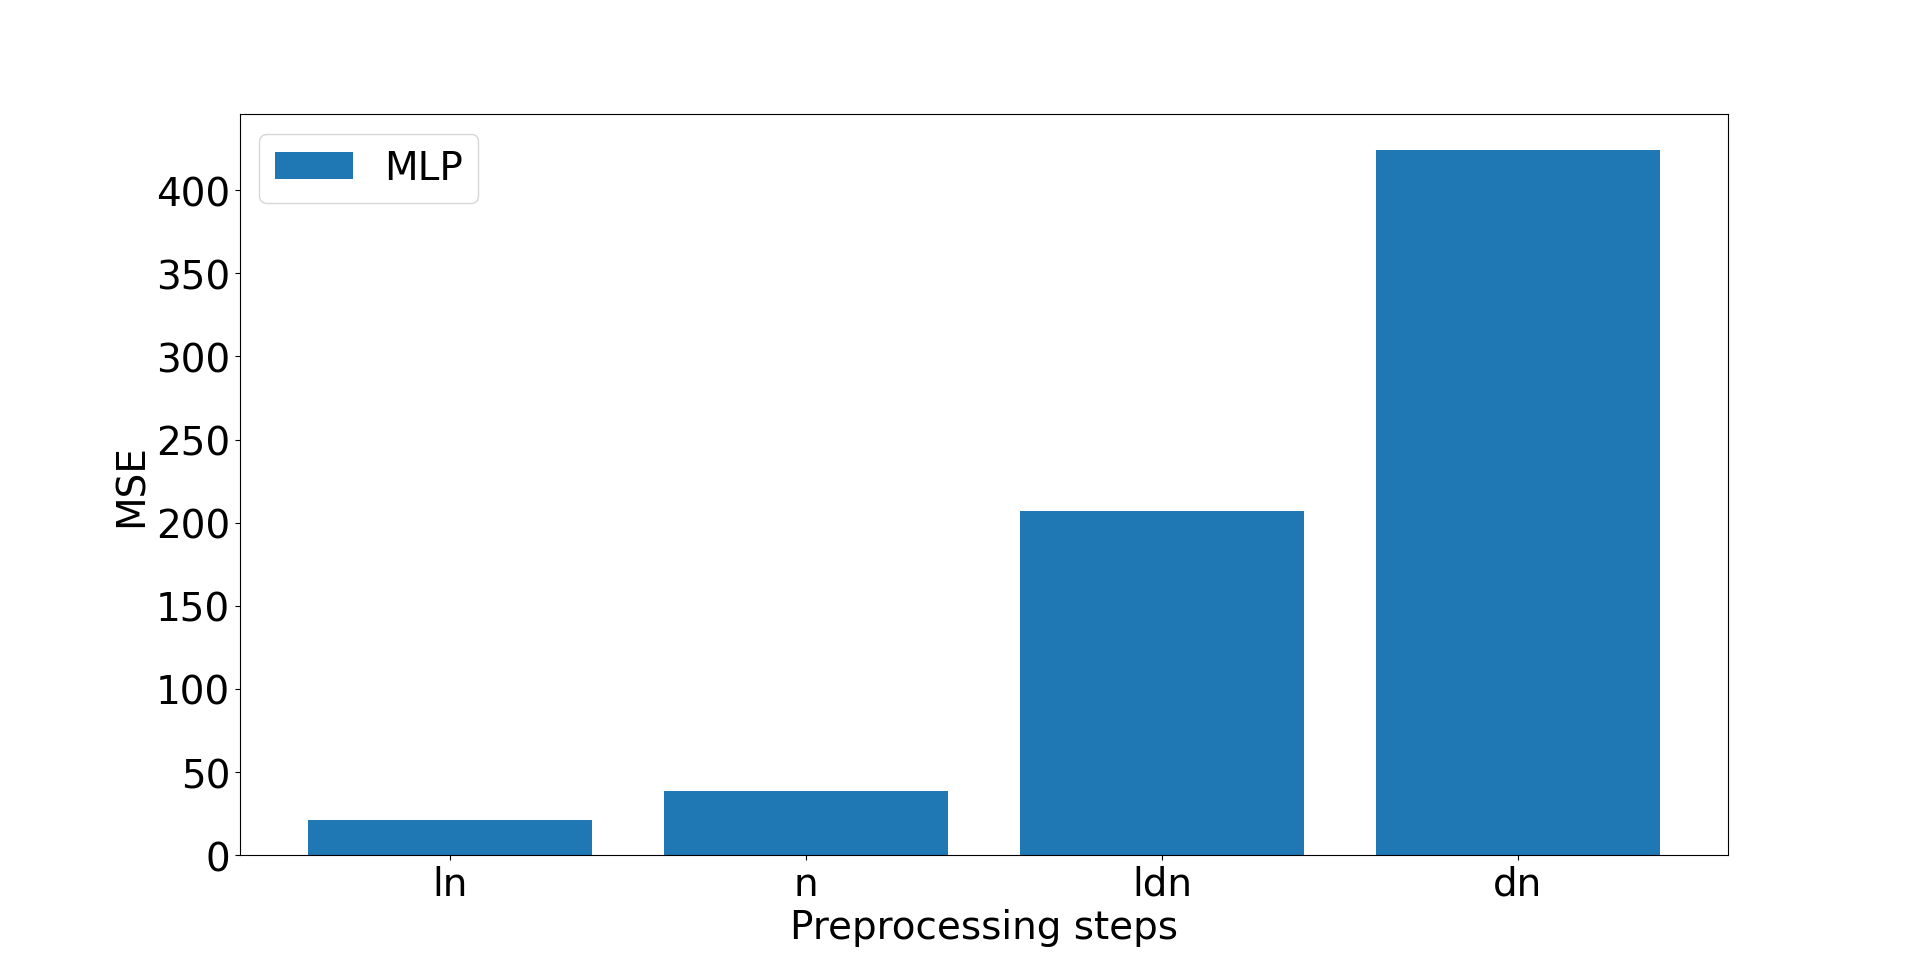
\includegraphics[width=\textwidth]{images/metrics-by-dataset/mlp_mse.png}
    \centering
    \caption{The \gls{mse} for the \gls{mlp} model for various preprocessing steps. The sets of processing steps are indicated in shorthand as follows: l - log transformed, d - differenced, n - normalized.}
    \label{fig:mlp-mse}
\end{figure}

\begin{figure}[h]
    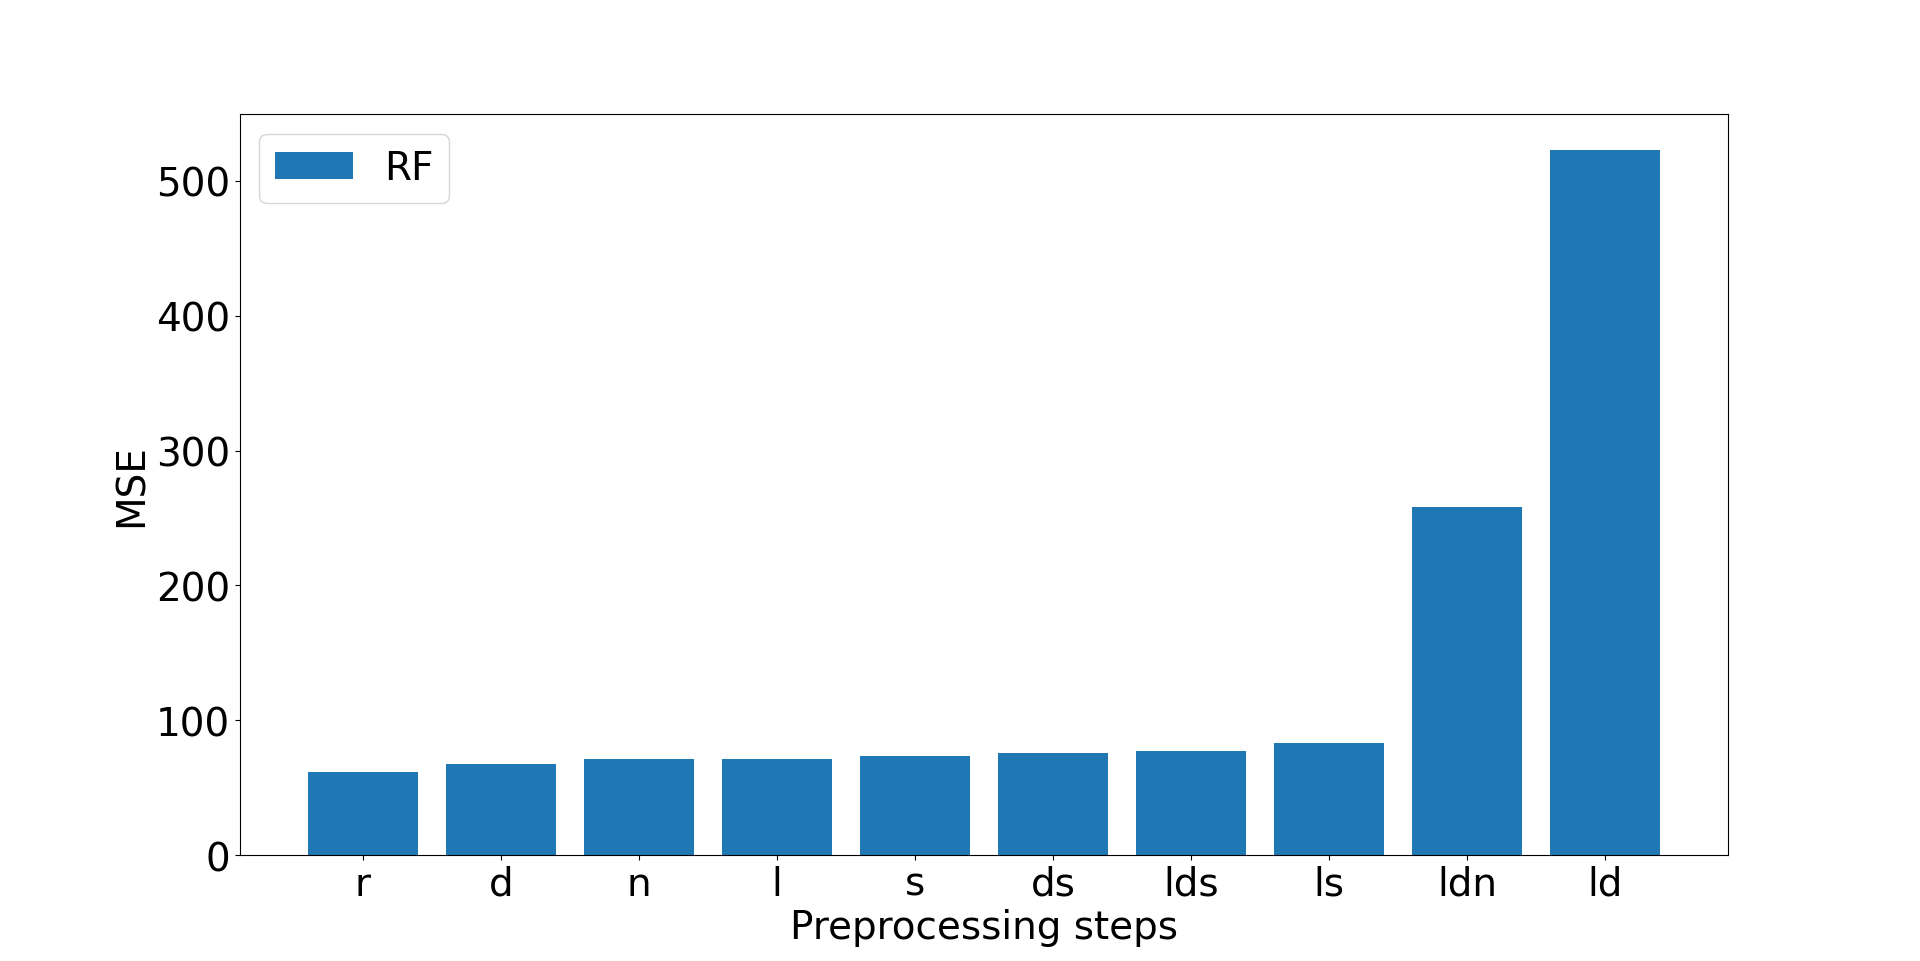
\includegraphics[width=\textwidth]{images/metrics-by-dataset/rf_mse.png}
    \centering
    \caption{The \gls{mse} for the \gls{rf} model for various preprocessing steps. The sets of processing steps are indicated in shorthand as follows: l - log transformed, d - differenced, n - normalized, s - standardized, r - raw.}
    \label{fig:rf-mse}
\end{figure}

\begin{figure}[h]
    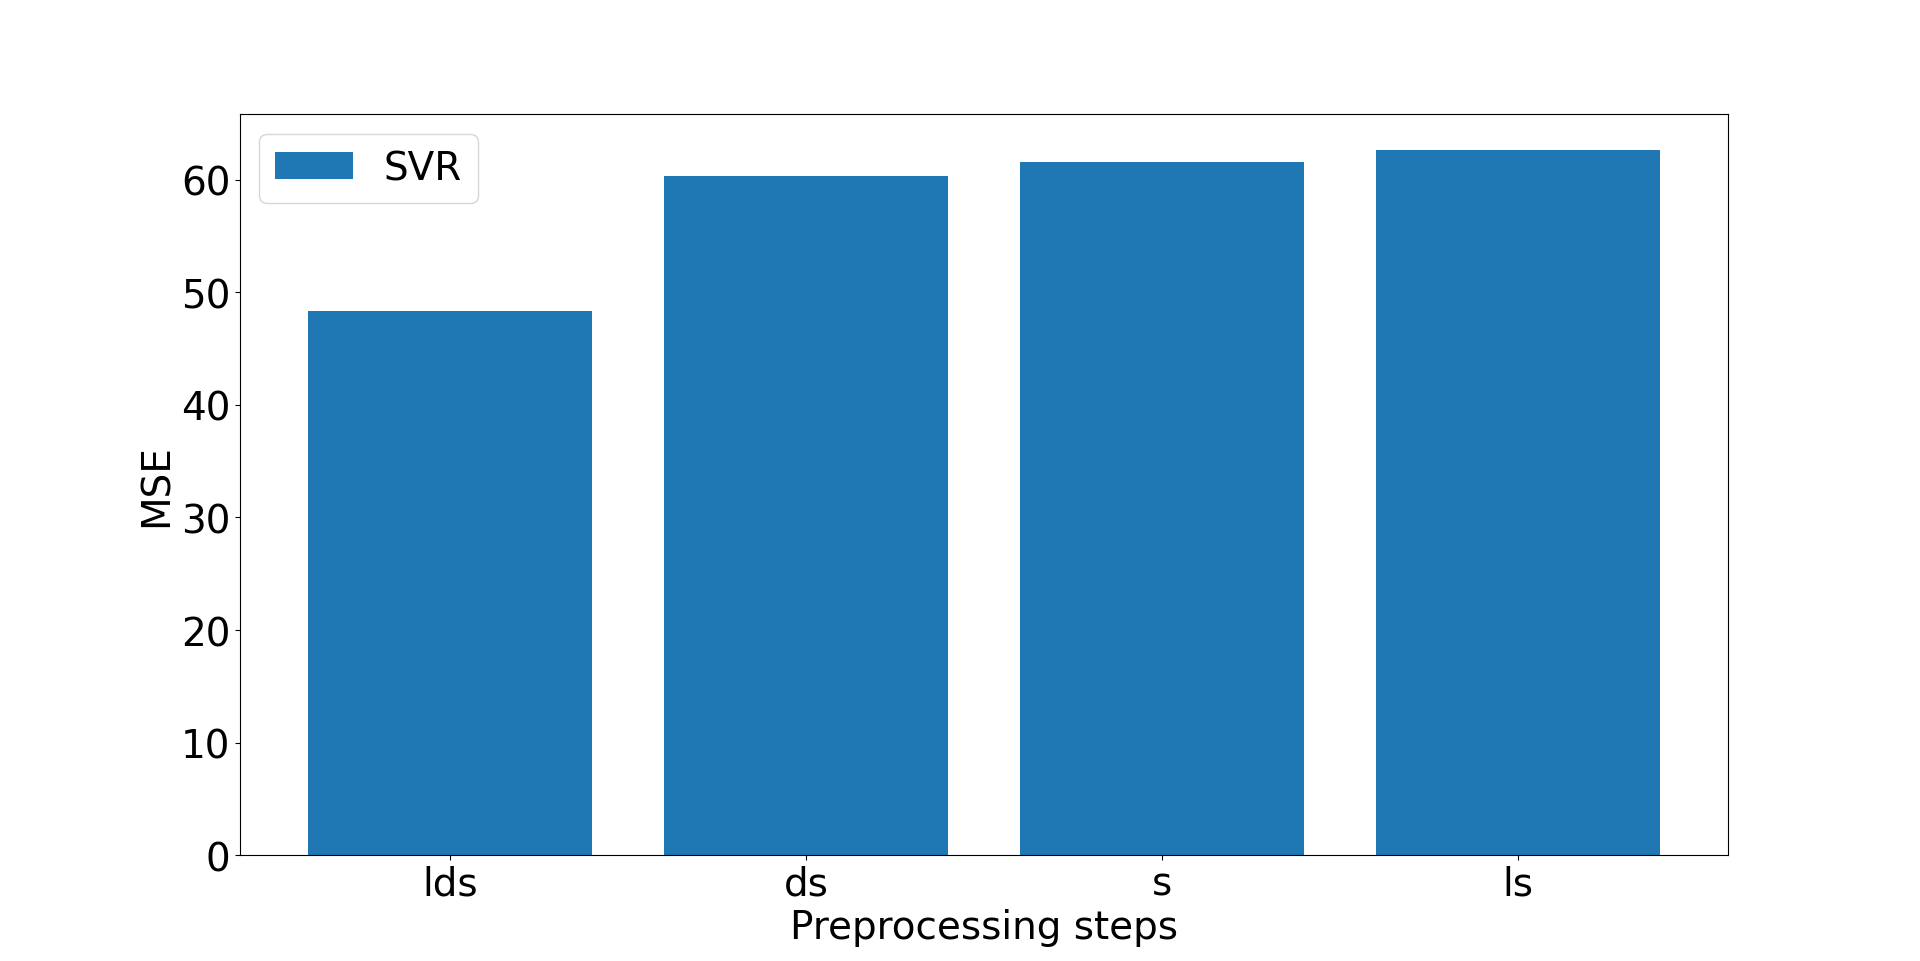
\includegraphics[width=\textwidth]{images/metrics-by-dataset/svr_mse.png}
    \centering
    \caption{The \gls{mse} for the \gls{svr} model for various preprocessing steps. The sets of processing steps are indicated in shorthand as follows: l - log transformed, d - differenced, s - standardized.}
    \label{fig:svr-mse}
\end{figure}

\begin{figure}[h]
    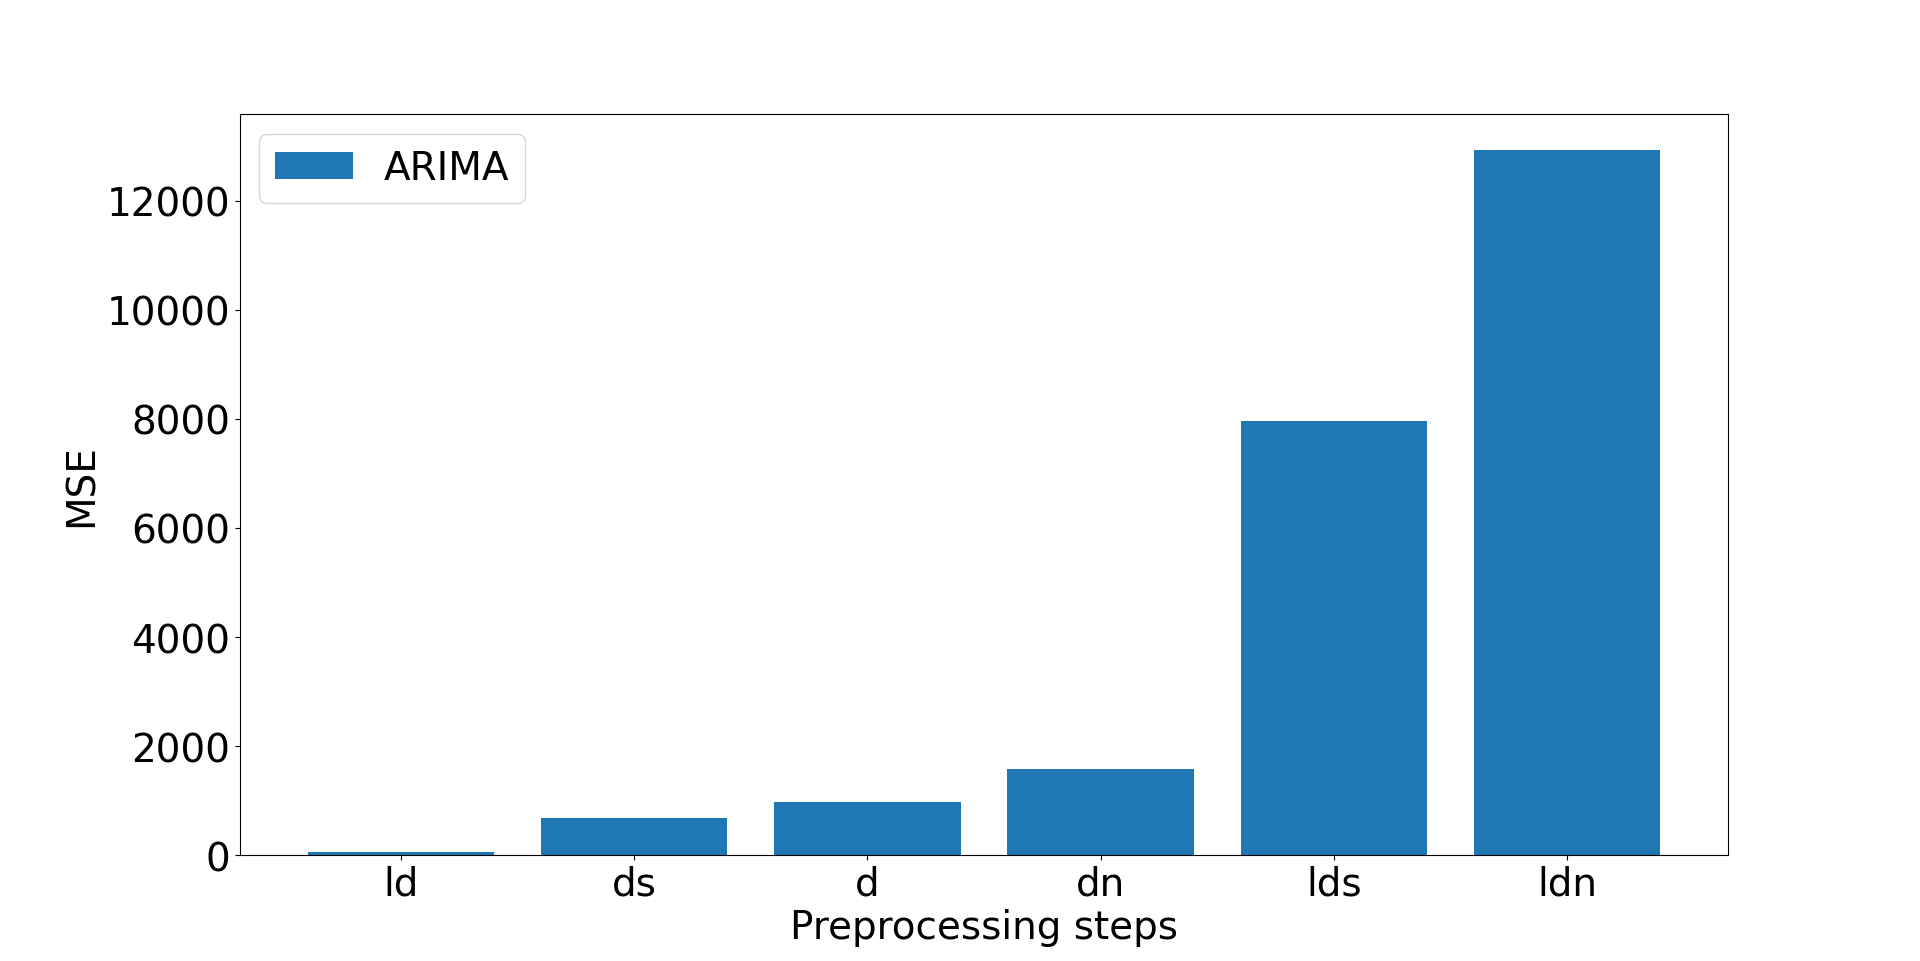
\includegraphics[width=\textwidth]{images/metrics-by-dataset/arima_mse.png}
    \centering
    \caption{The \gls{mse} for the \gls{arima} model for various preprocessing steps. The sets of processing steps are indicated in shorthand as follows: l - log transformed, d - differenced, n - normalized, s - standardized, r - raw.}
    \label{fig:arima-mse}
\end{figure}

On the basis of the created rankings the best dataset preprocessing variations for each model were selected. The results are displayed in table \ref{tab:best-datasets}.

% Metric - Model - Preprocessing steps
% mse - mlp - log-normalized
% hitrate - mlp - log-diff-normalized
% mse - rf - raw
% hitrate - rf - log-transformed
% mse - svr - log-diff-standardized
% hitrate - svr - log-diff-standardized

\begin{table}[h]
    \centering
    \caption{The best dataset preprocessing steps per model by \gls{mse}.}
    \begin{tabular}{|c|c|}
        \hline
        Model & Preprocessing Steps \\
        \hline
        \hline
        \gls{mlp} & log-normalized \\
        \hline
        \gls{rf} & raw \\
        \hline
        \gls{svr} & log-diff-standardized \\
        \hline
        \gls{arima} & log-differenced \\
        \hline
    \end{tabular}
    \label{tab:best-datasets}
\end{table}

\newpage

For the purpose of comparing the overall performance of different models the average \gls{mse} over both the train and test sets over all offsets was calculated. The results are visible in the bar chart in figure \ref{fig:mse-model-cmp}.

% Bar chart comparison of the best performing models

\begin{figure}[h]
    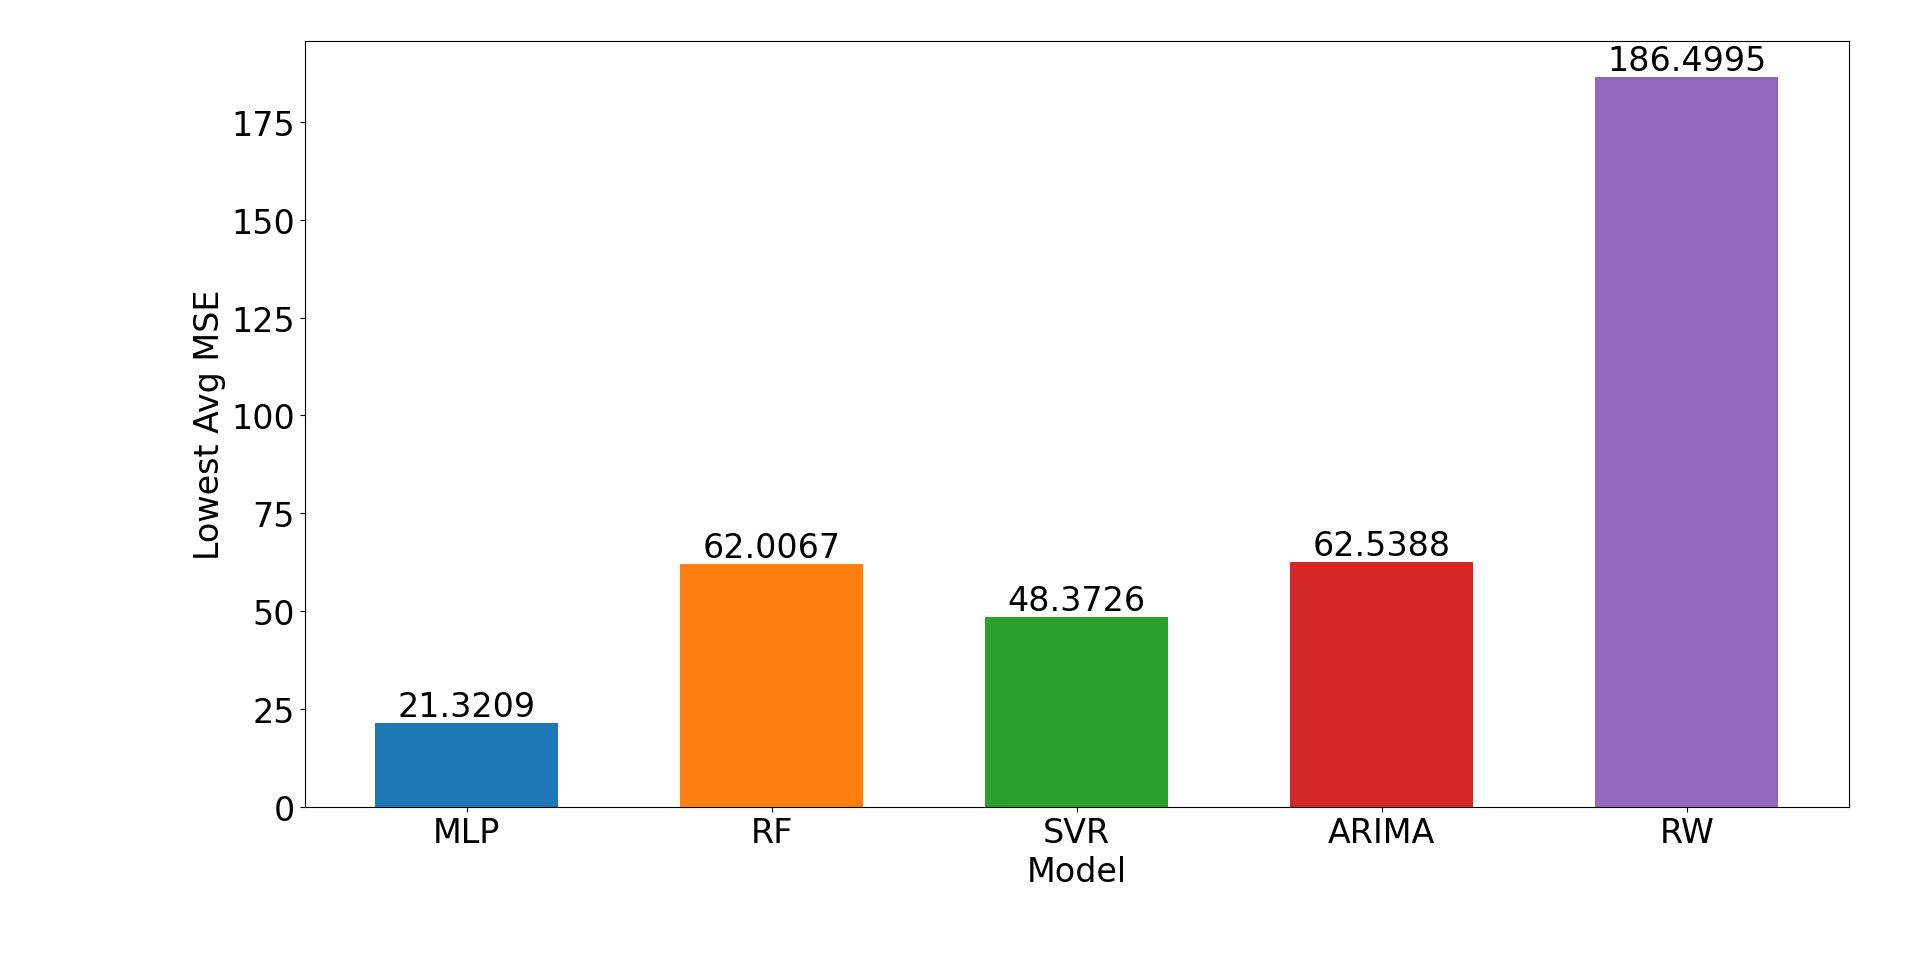
\includegraphics[width=\textwidth]{images/metrics-by-model/mse.png}
    \centering
    \caption{Comparison of the lowest cumulative average of the average \gls{mse} over train and test sets of all offset forecasts for the best dataset preprocessing variant for each model.}
    \label{fig:mse-model-cmp}
\end{figure}

\subsection{Forecasts}\label{Forecasts}

In the next step a cumulative bar chart of the \gls{mse} shown in figure \ref{fig:cumulative-mse} of the forecasts was created to illustrate the relative performance of each model on the basis of it's best dataset preprocessing variant for each offset.

% Bar charts of the offset dependant mse and hitrate of various forecasts

\begin{figure}[h]
    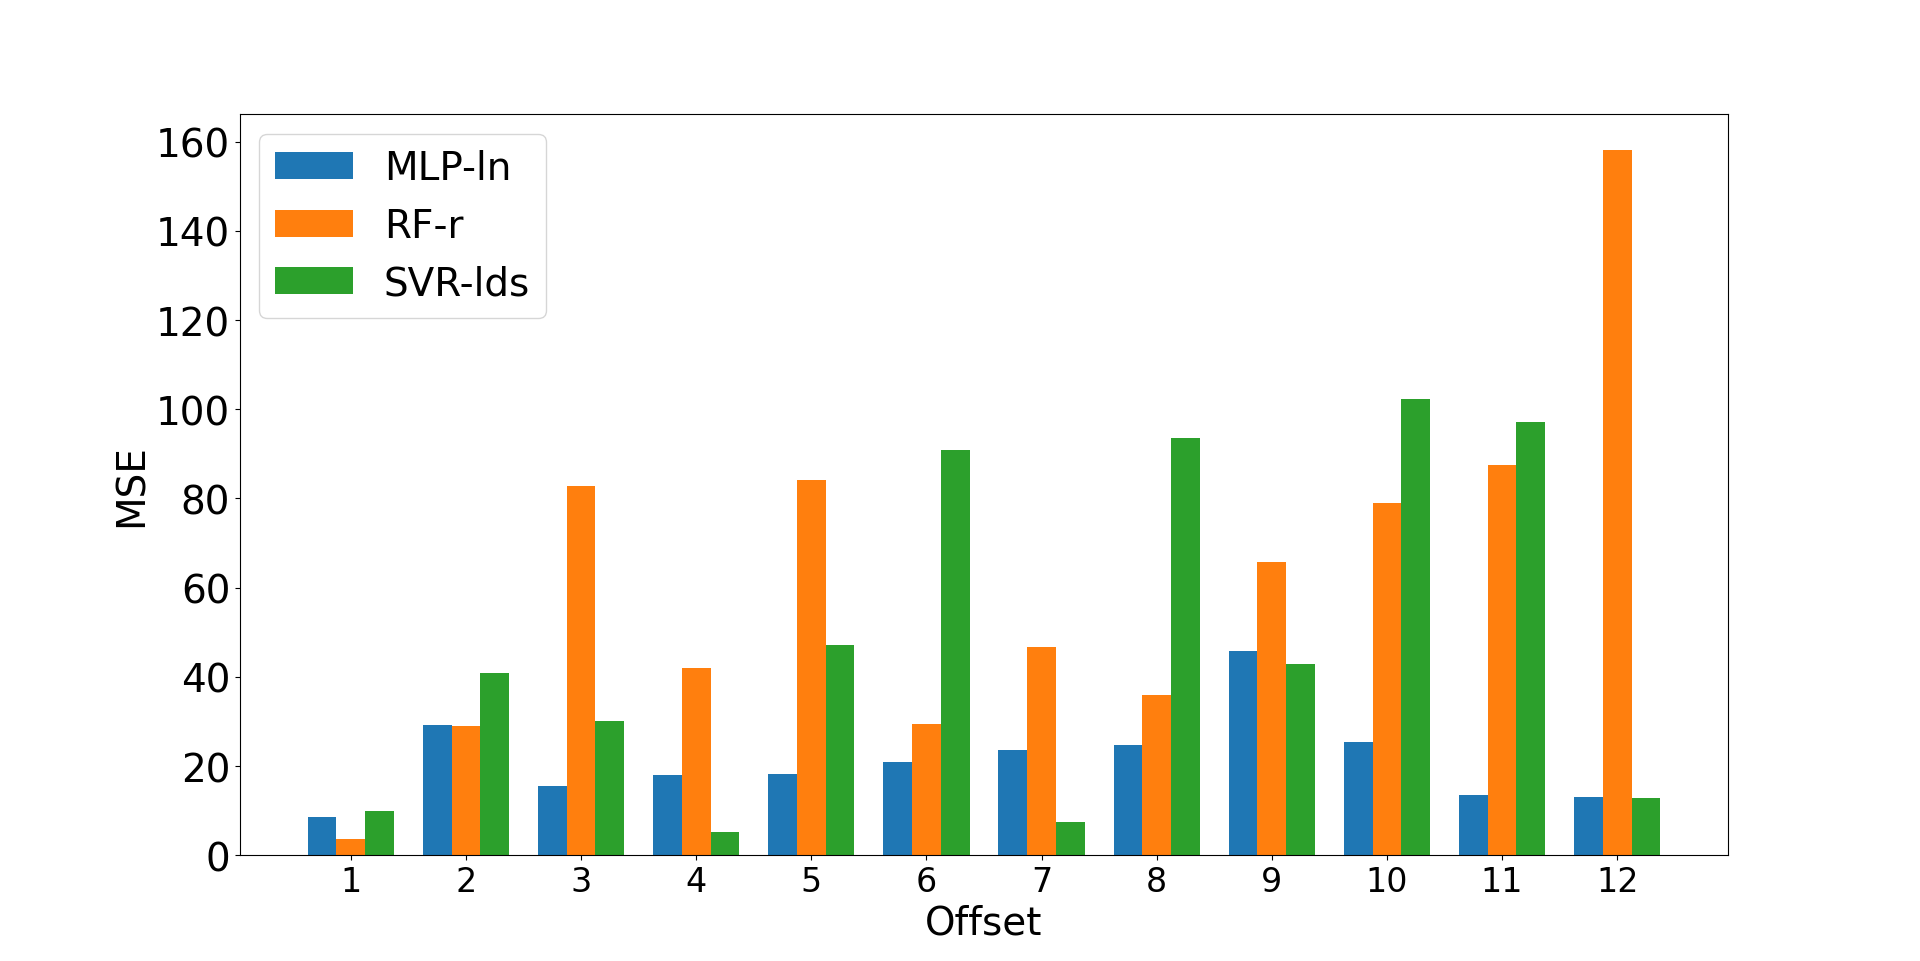
\includegraphics[width=\textwidth]{images/metrics-by-offset/all-mse.png}
    \centering
    \caption{Comparison of the \gls{mse} of the forecasts for the best dataset preprocessing variant for each model for each offset. The sets of processing steps are indicated in shorthand as follows: l - log transformed, d - differenced, n - normalized, s - standardized, r - raw.}
    \label{fig:cumulative-mse}
\end{figure}

Additionally as can be seen below in figures from \ref{fig:forecast-cmp-1} to \ref{fig:forecast-cmp-12} the reverse transformed forecasts for each model for the USD currency were plotted for each offset.

\begin{figure}[h]
    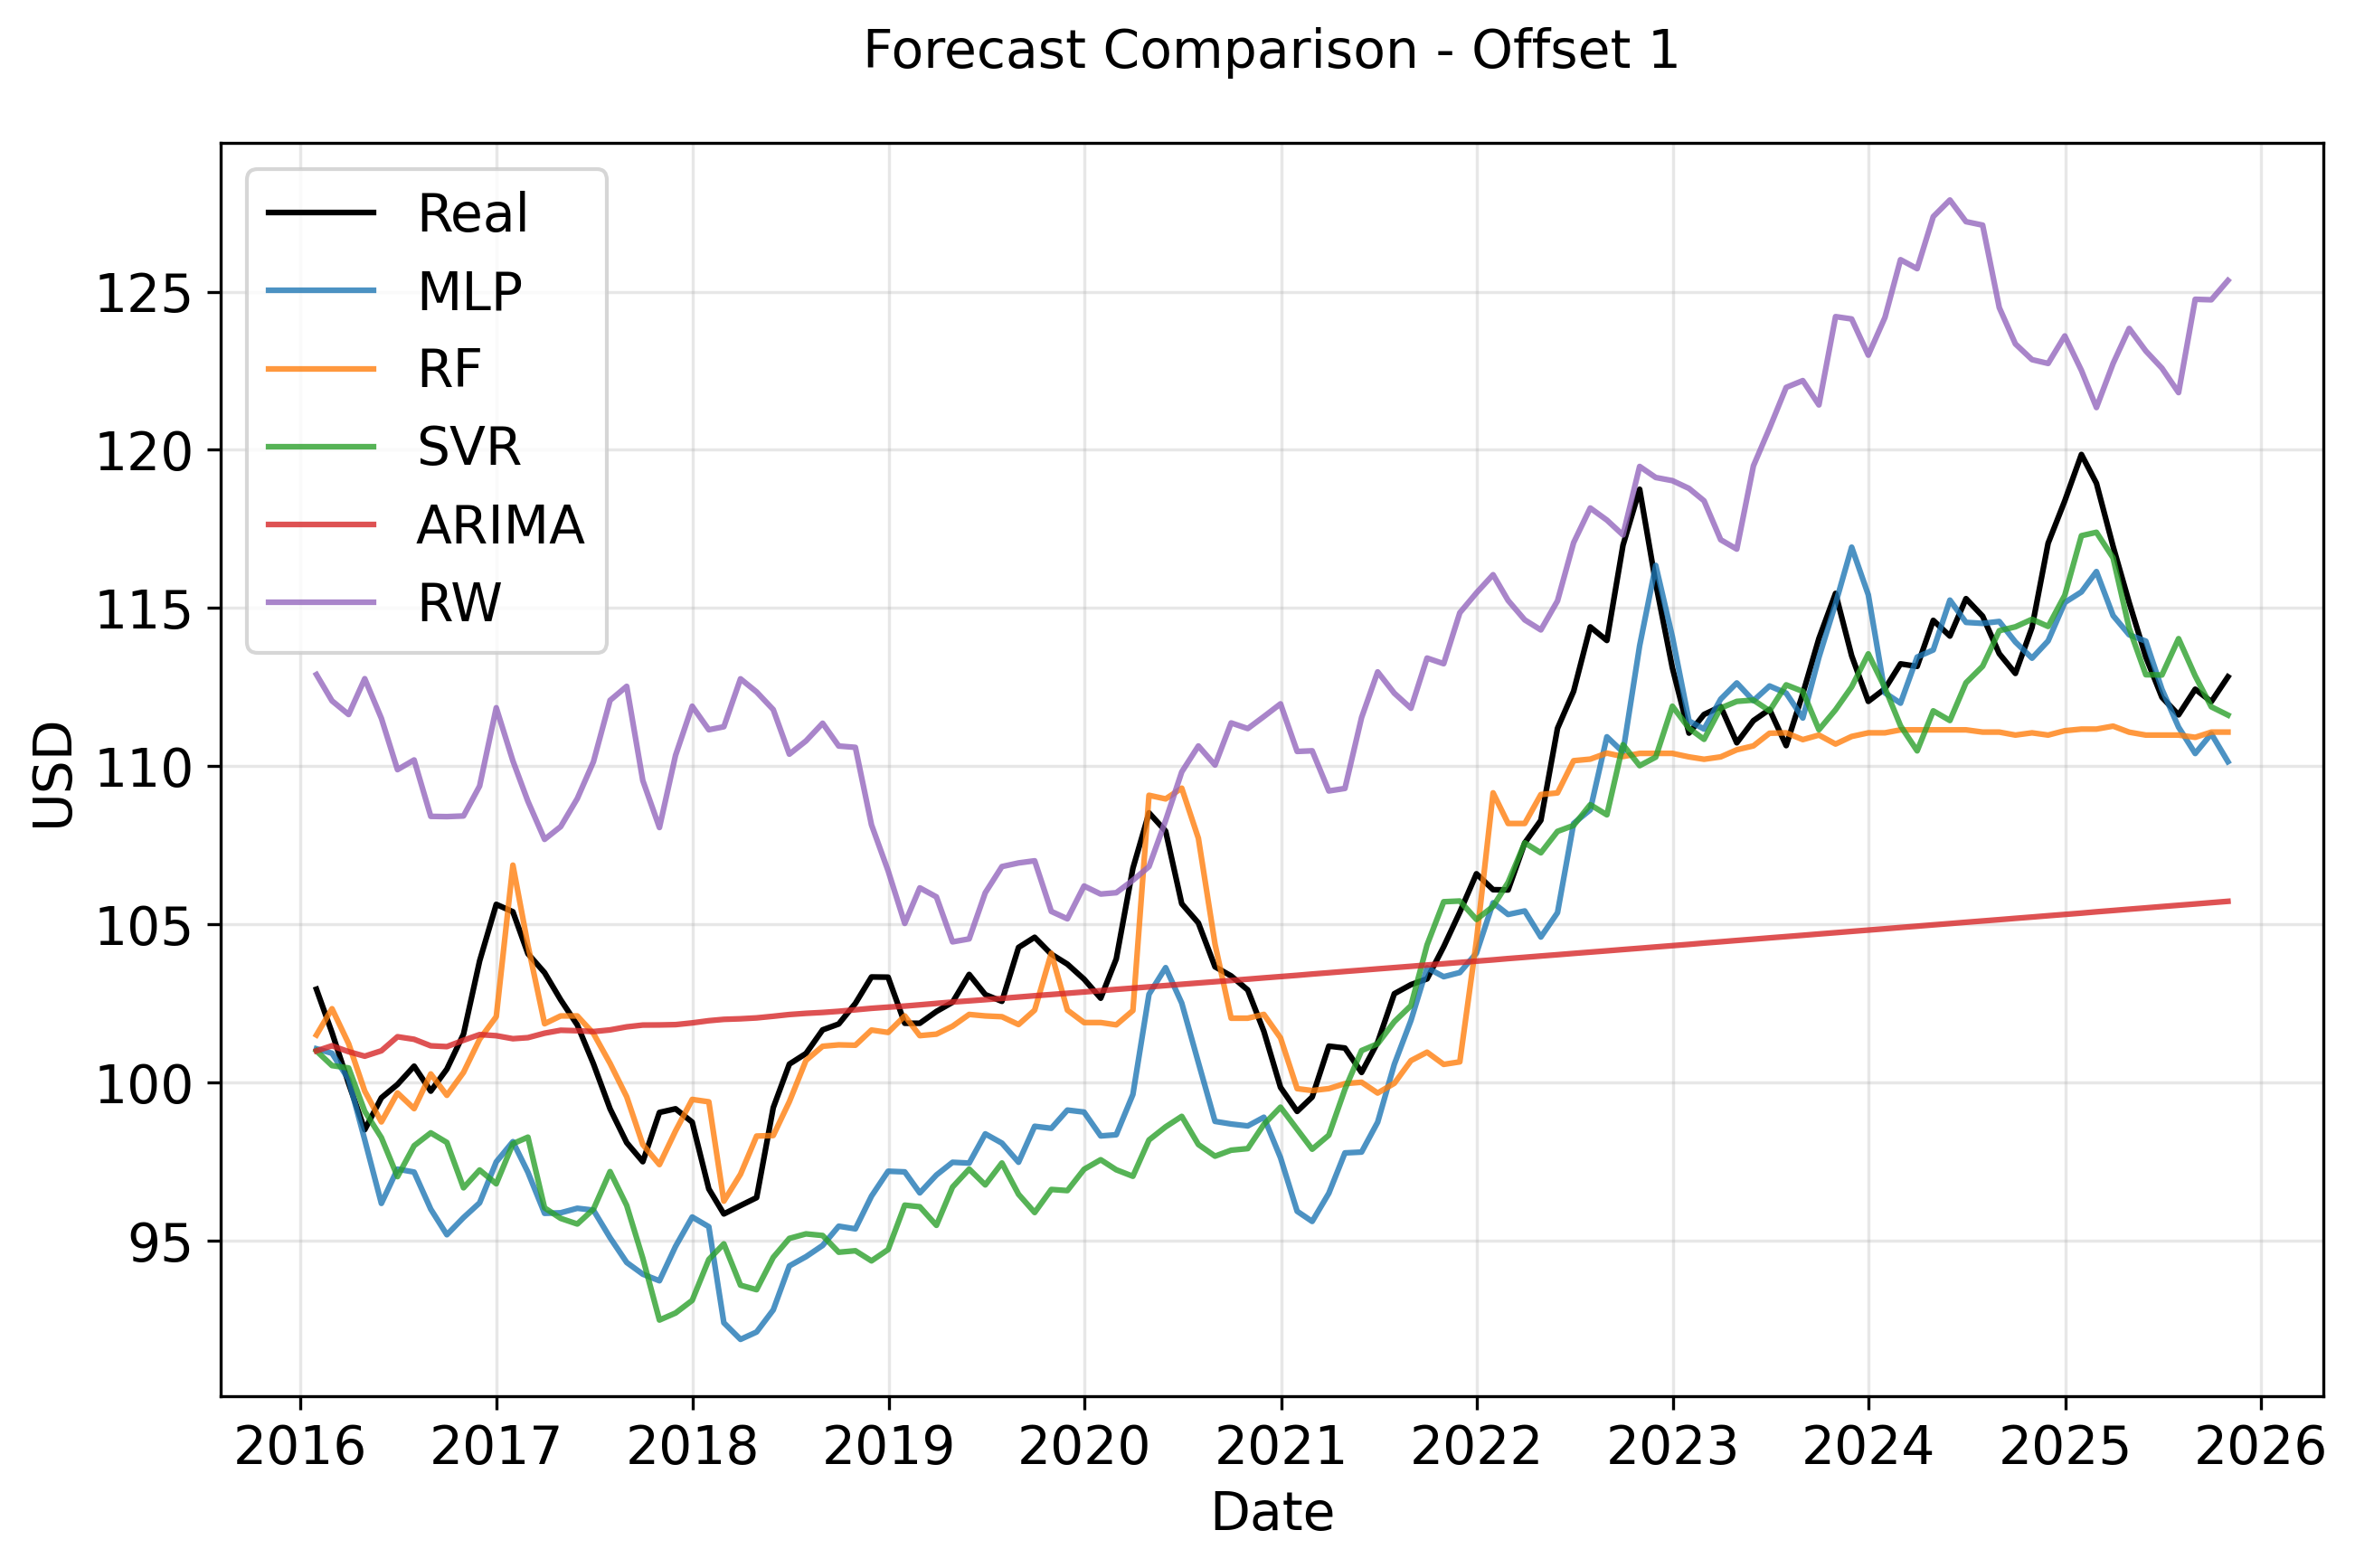
\includegraphics[width=\textwidth]{images/forecast-comparison/mse/1.png}
    \centering
    \caption{The best \gls{mse} forecasts per selected dataset per model for an offset of 1 month.}
    \label{fig:forecast-cmp-1}
\end{figure}

\begin{figure}[h]
    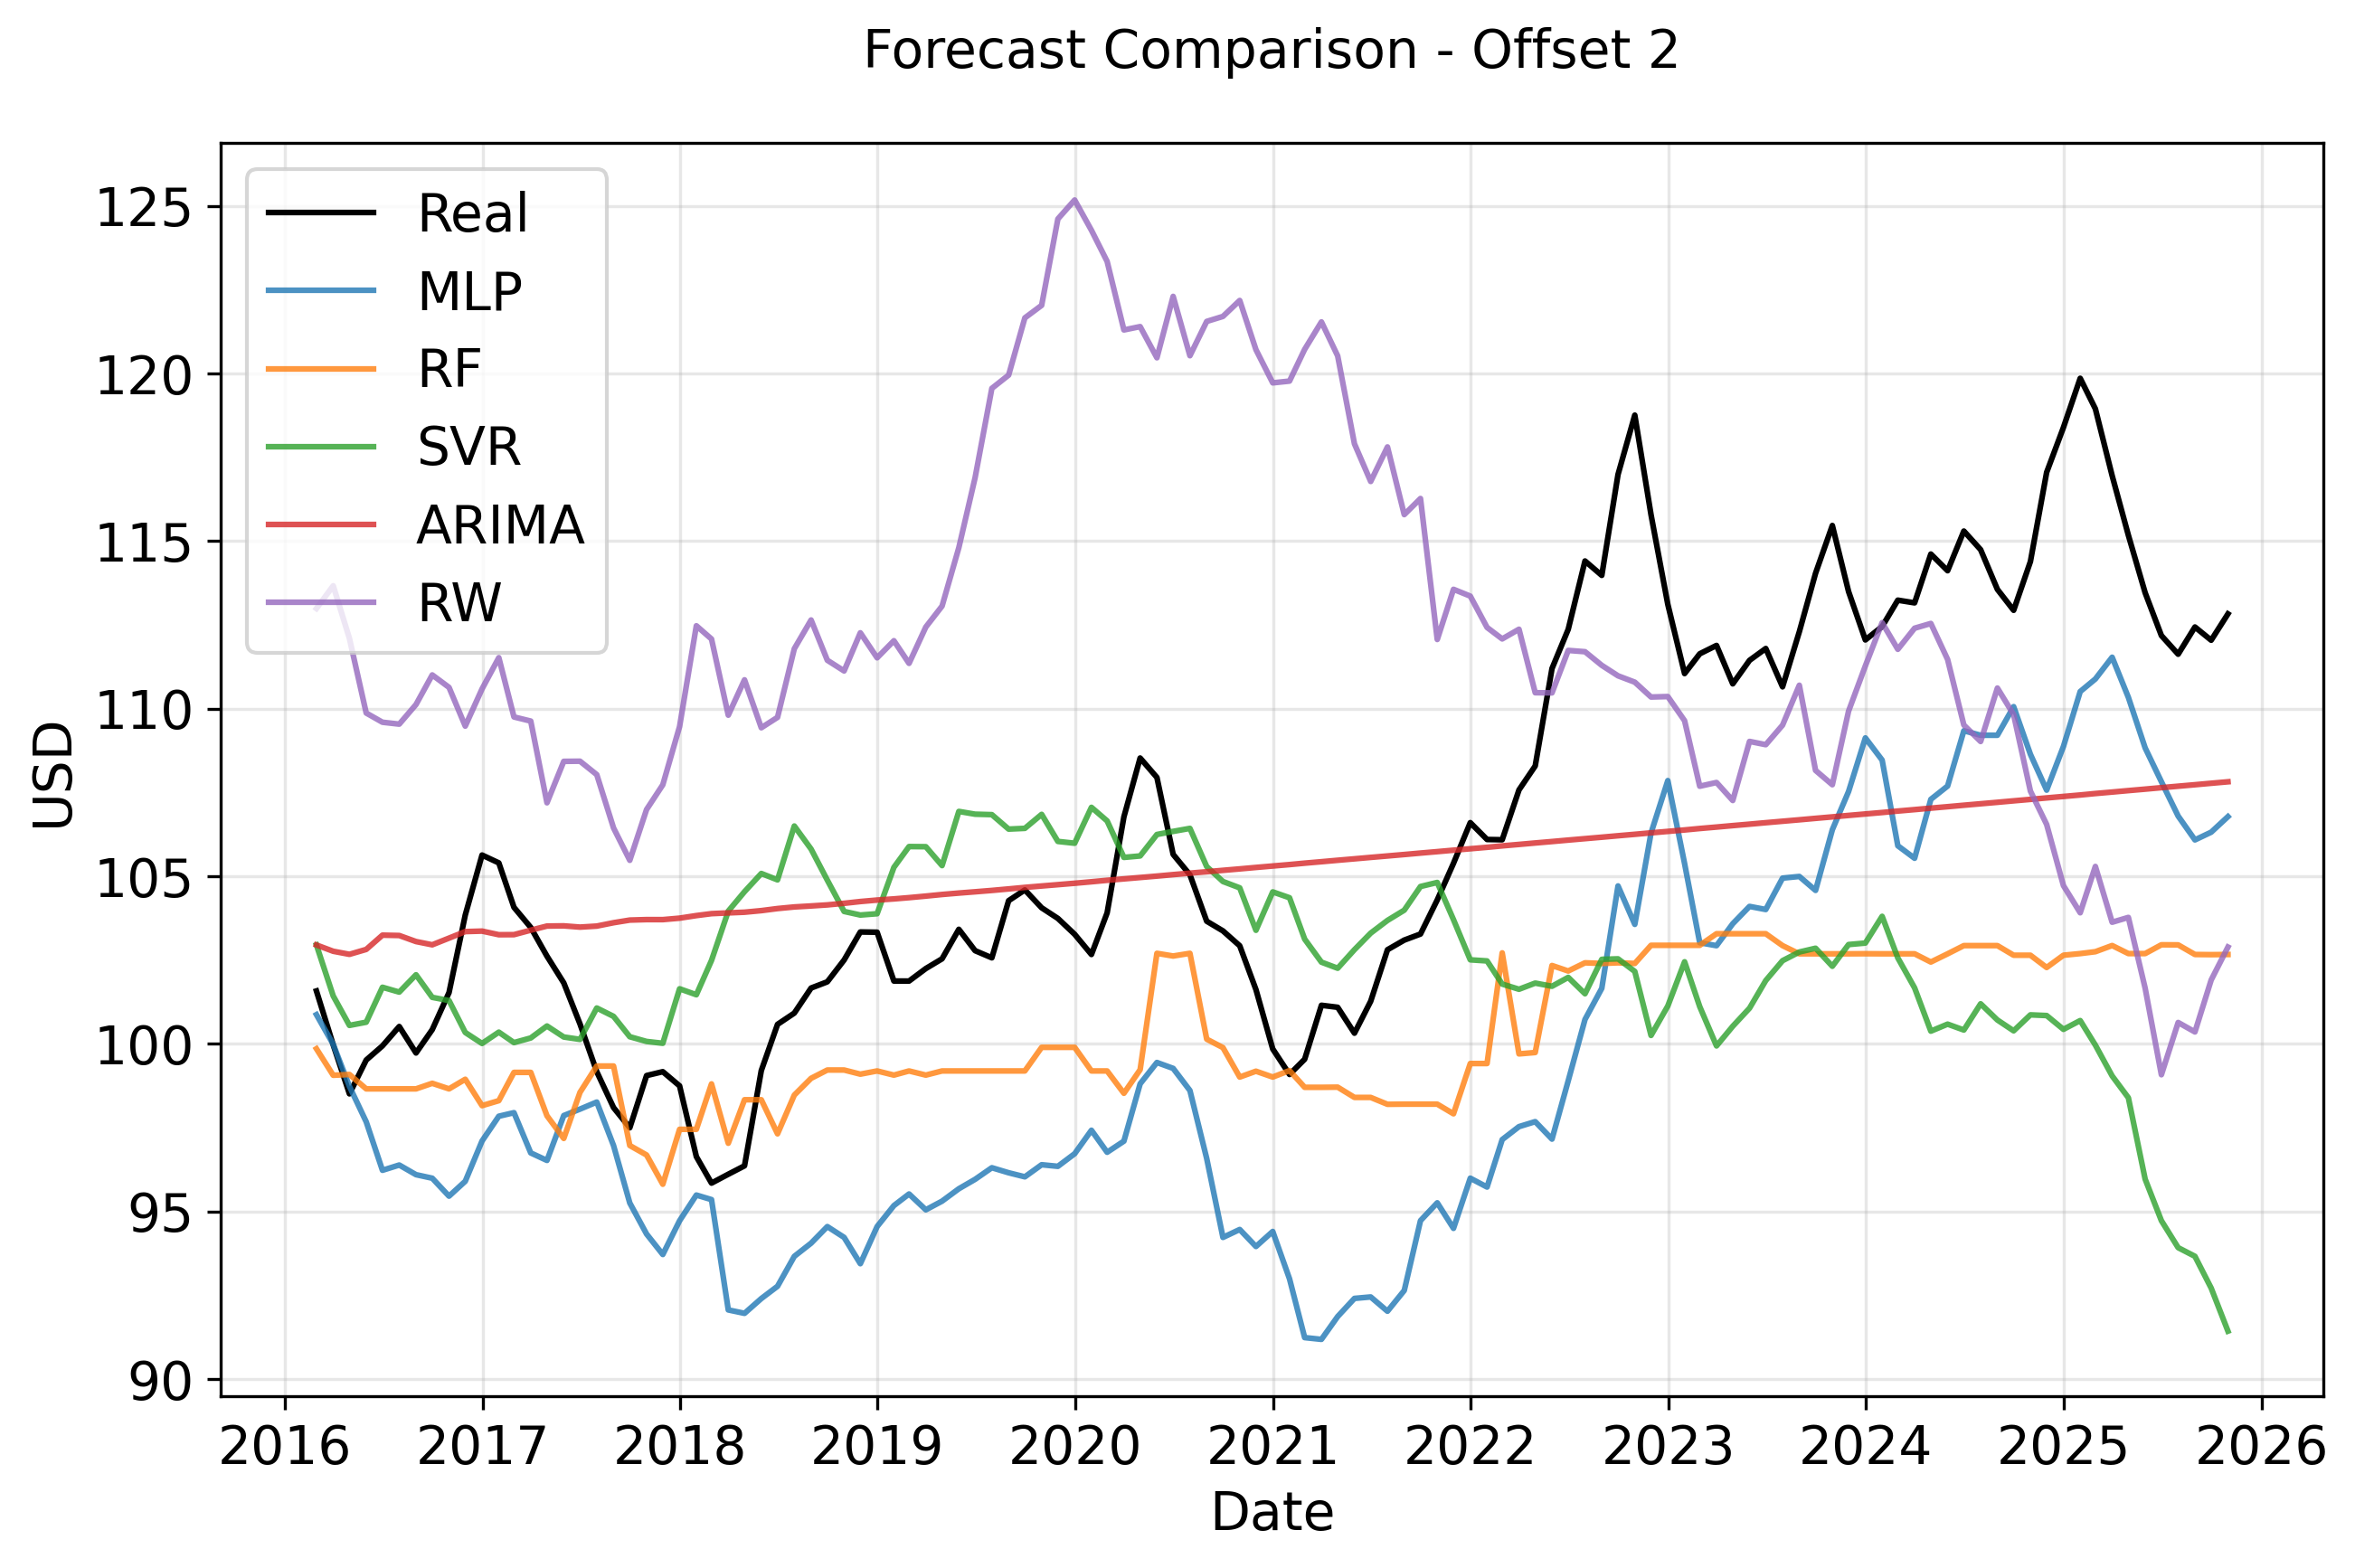
\includegraphics[width=\textwidth]{images/forecast-comparison/mse/2.png}
    \centering
    \caption{The best \gls{mse} forecasts per selected dataset per model for an offset of 2 months.}
    \label{fig:forecast-cmp-2}
\end{figure}

\begin{figure}[h]
    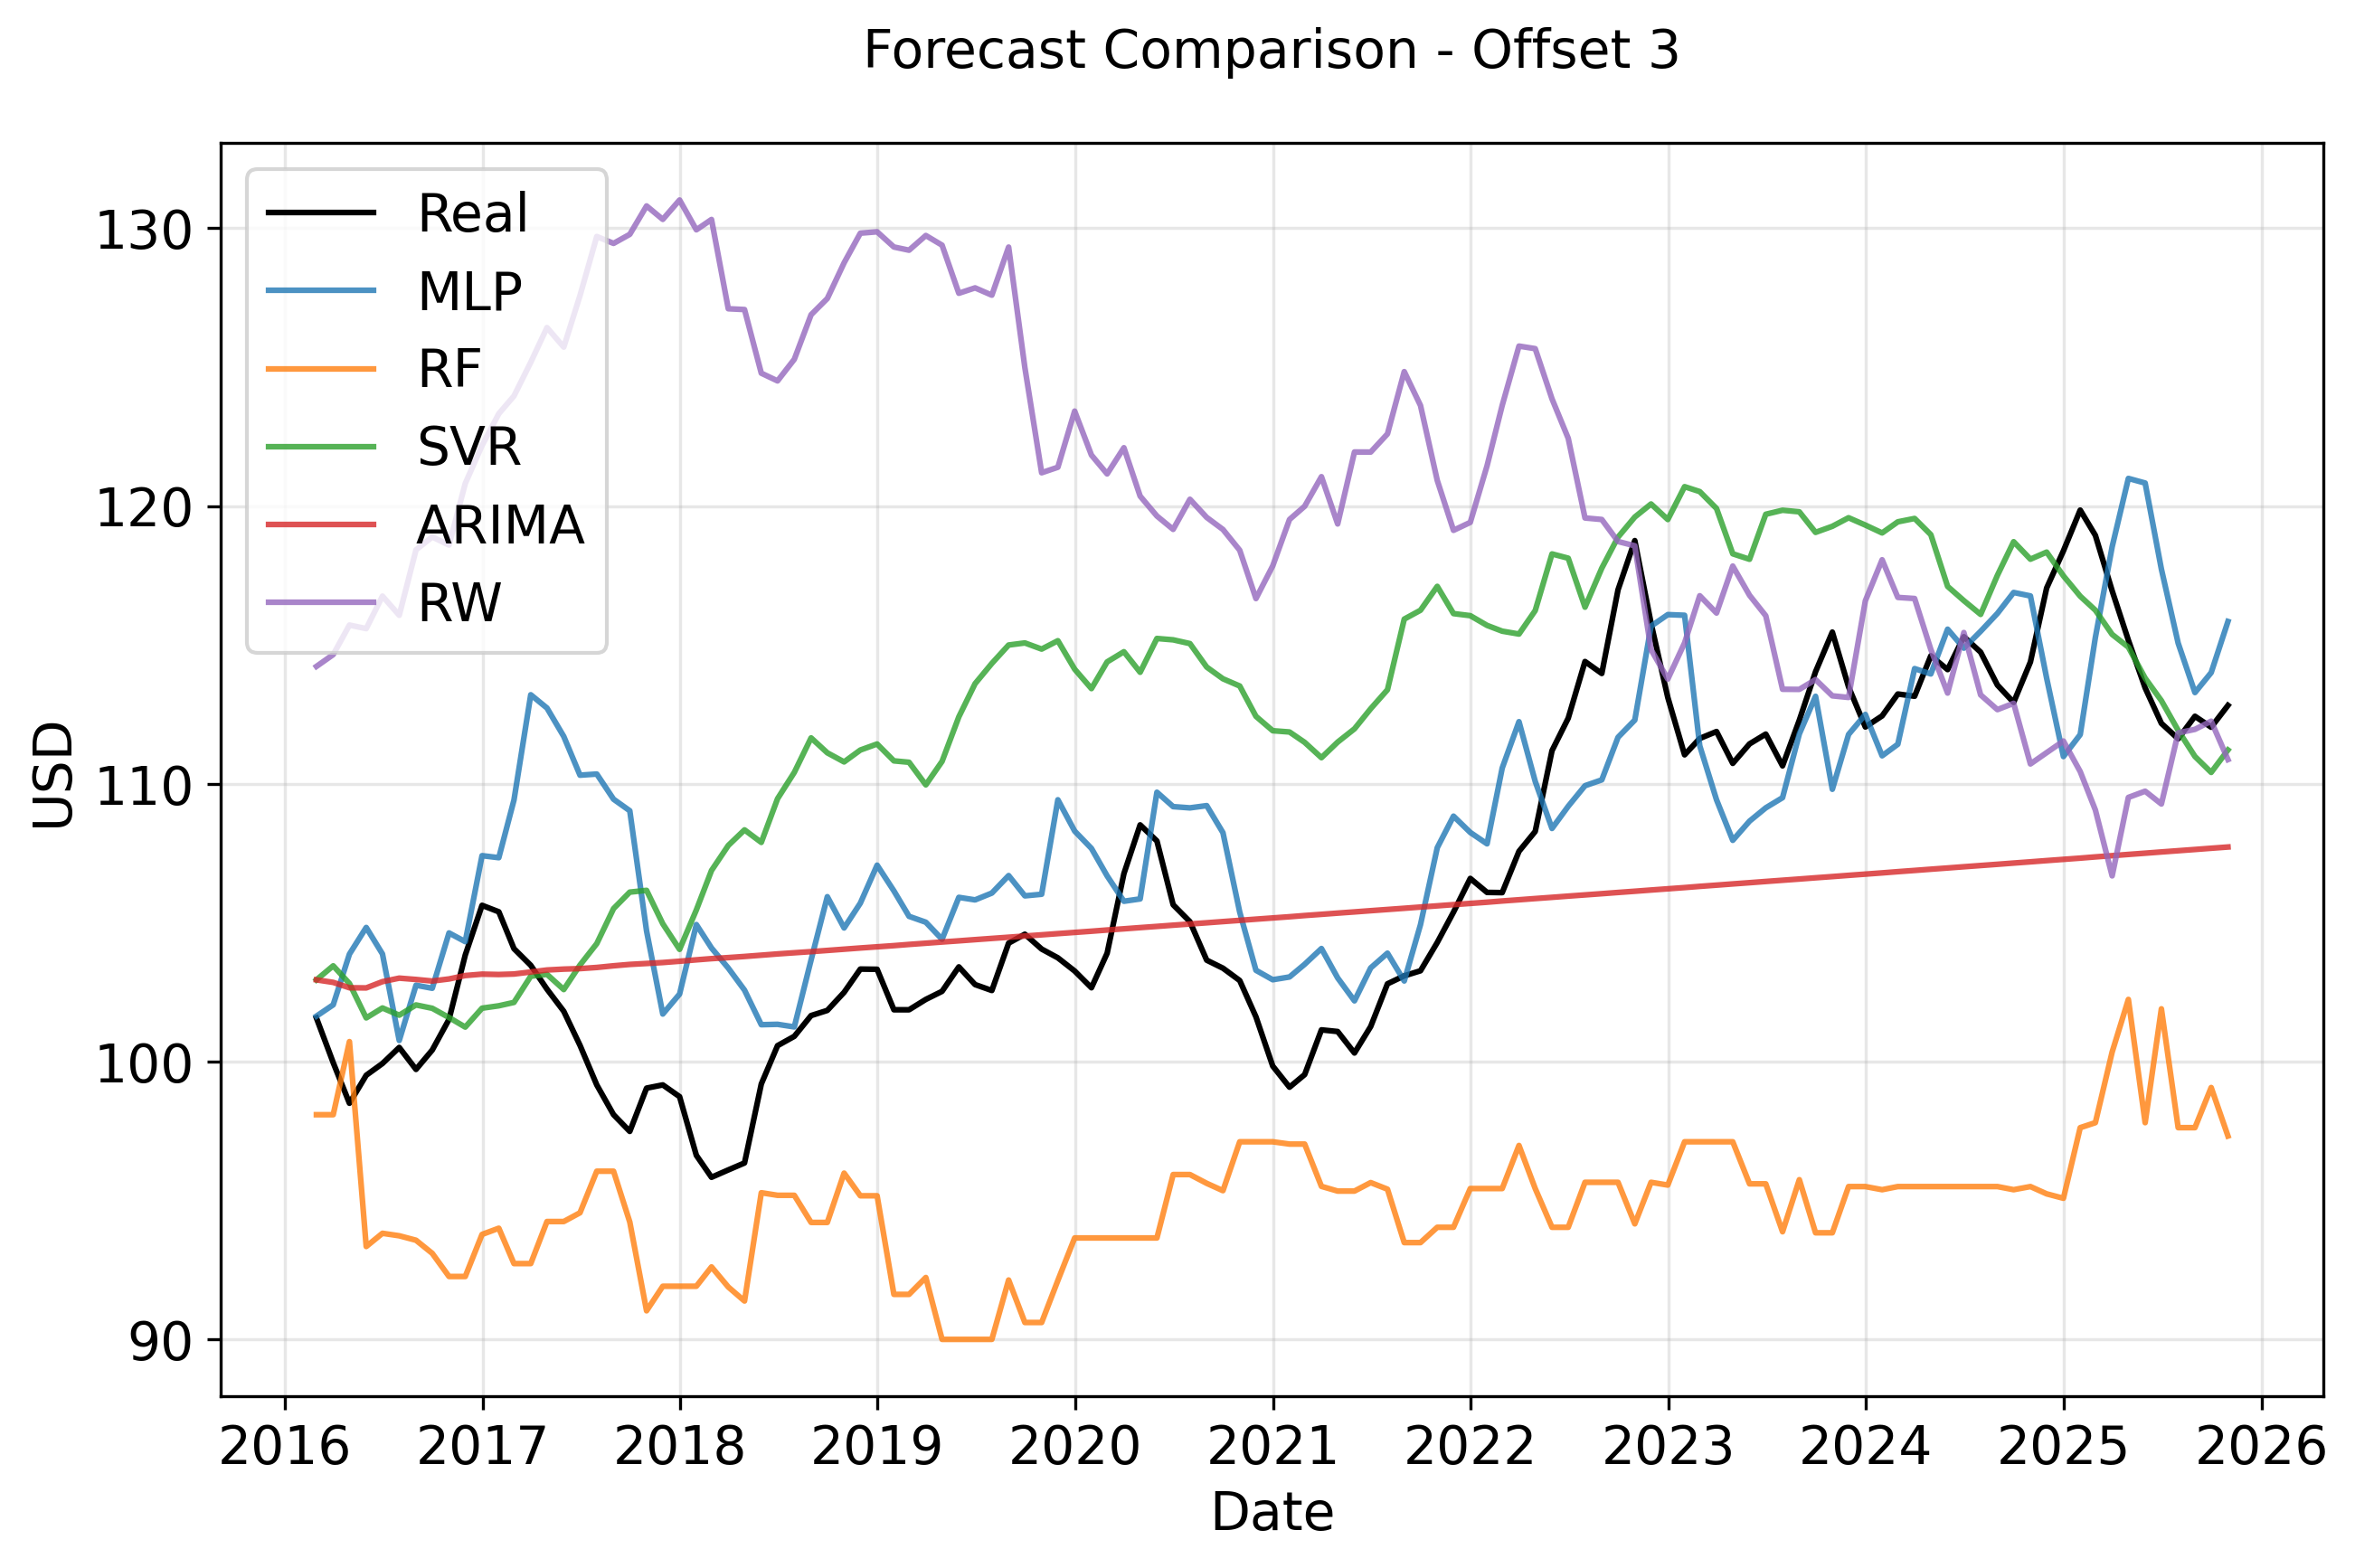
\includegraphics[width=\textwidth]{images/forecast-comparison/mse/3.png}
    \centering
    \caption{The best \gls{mse} forecasts per selected dataset per model for an offset of 3 months.}
    \label{fig:forecast-cmp-3}
\end{figure}

\begin{figure}[h]
    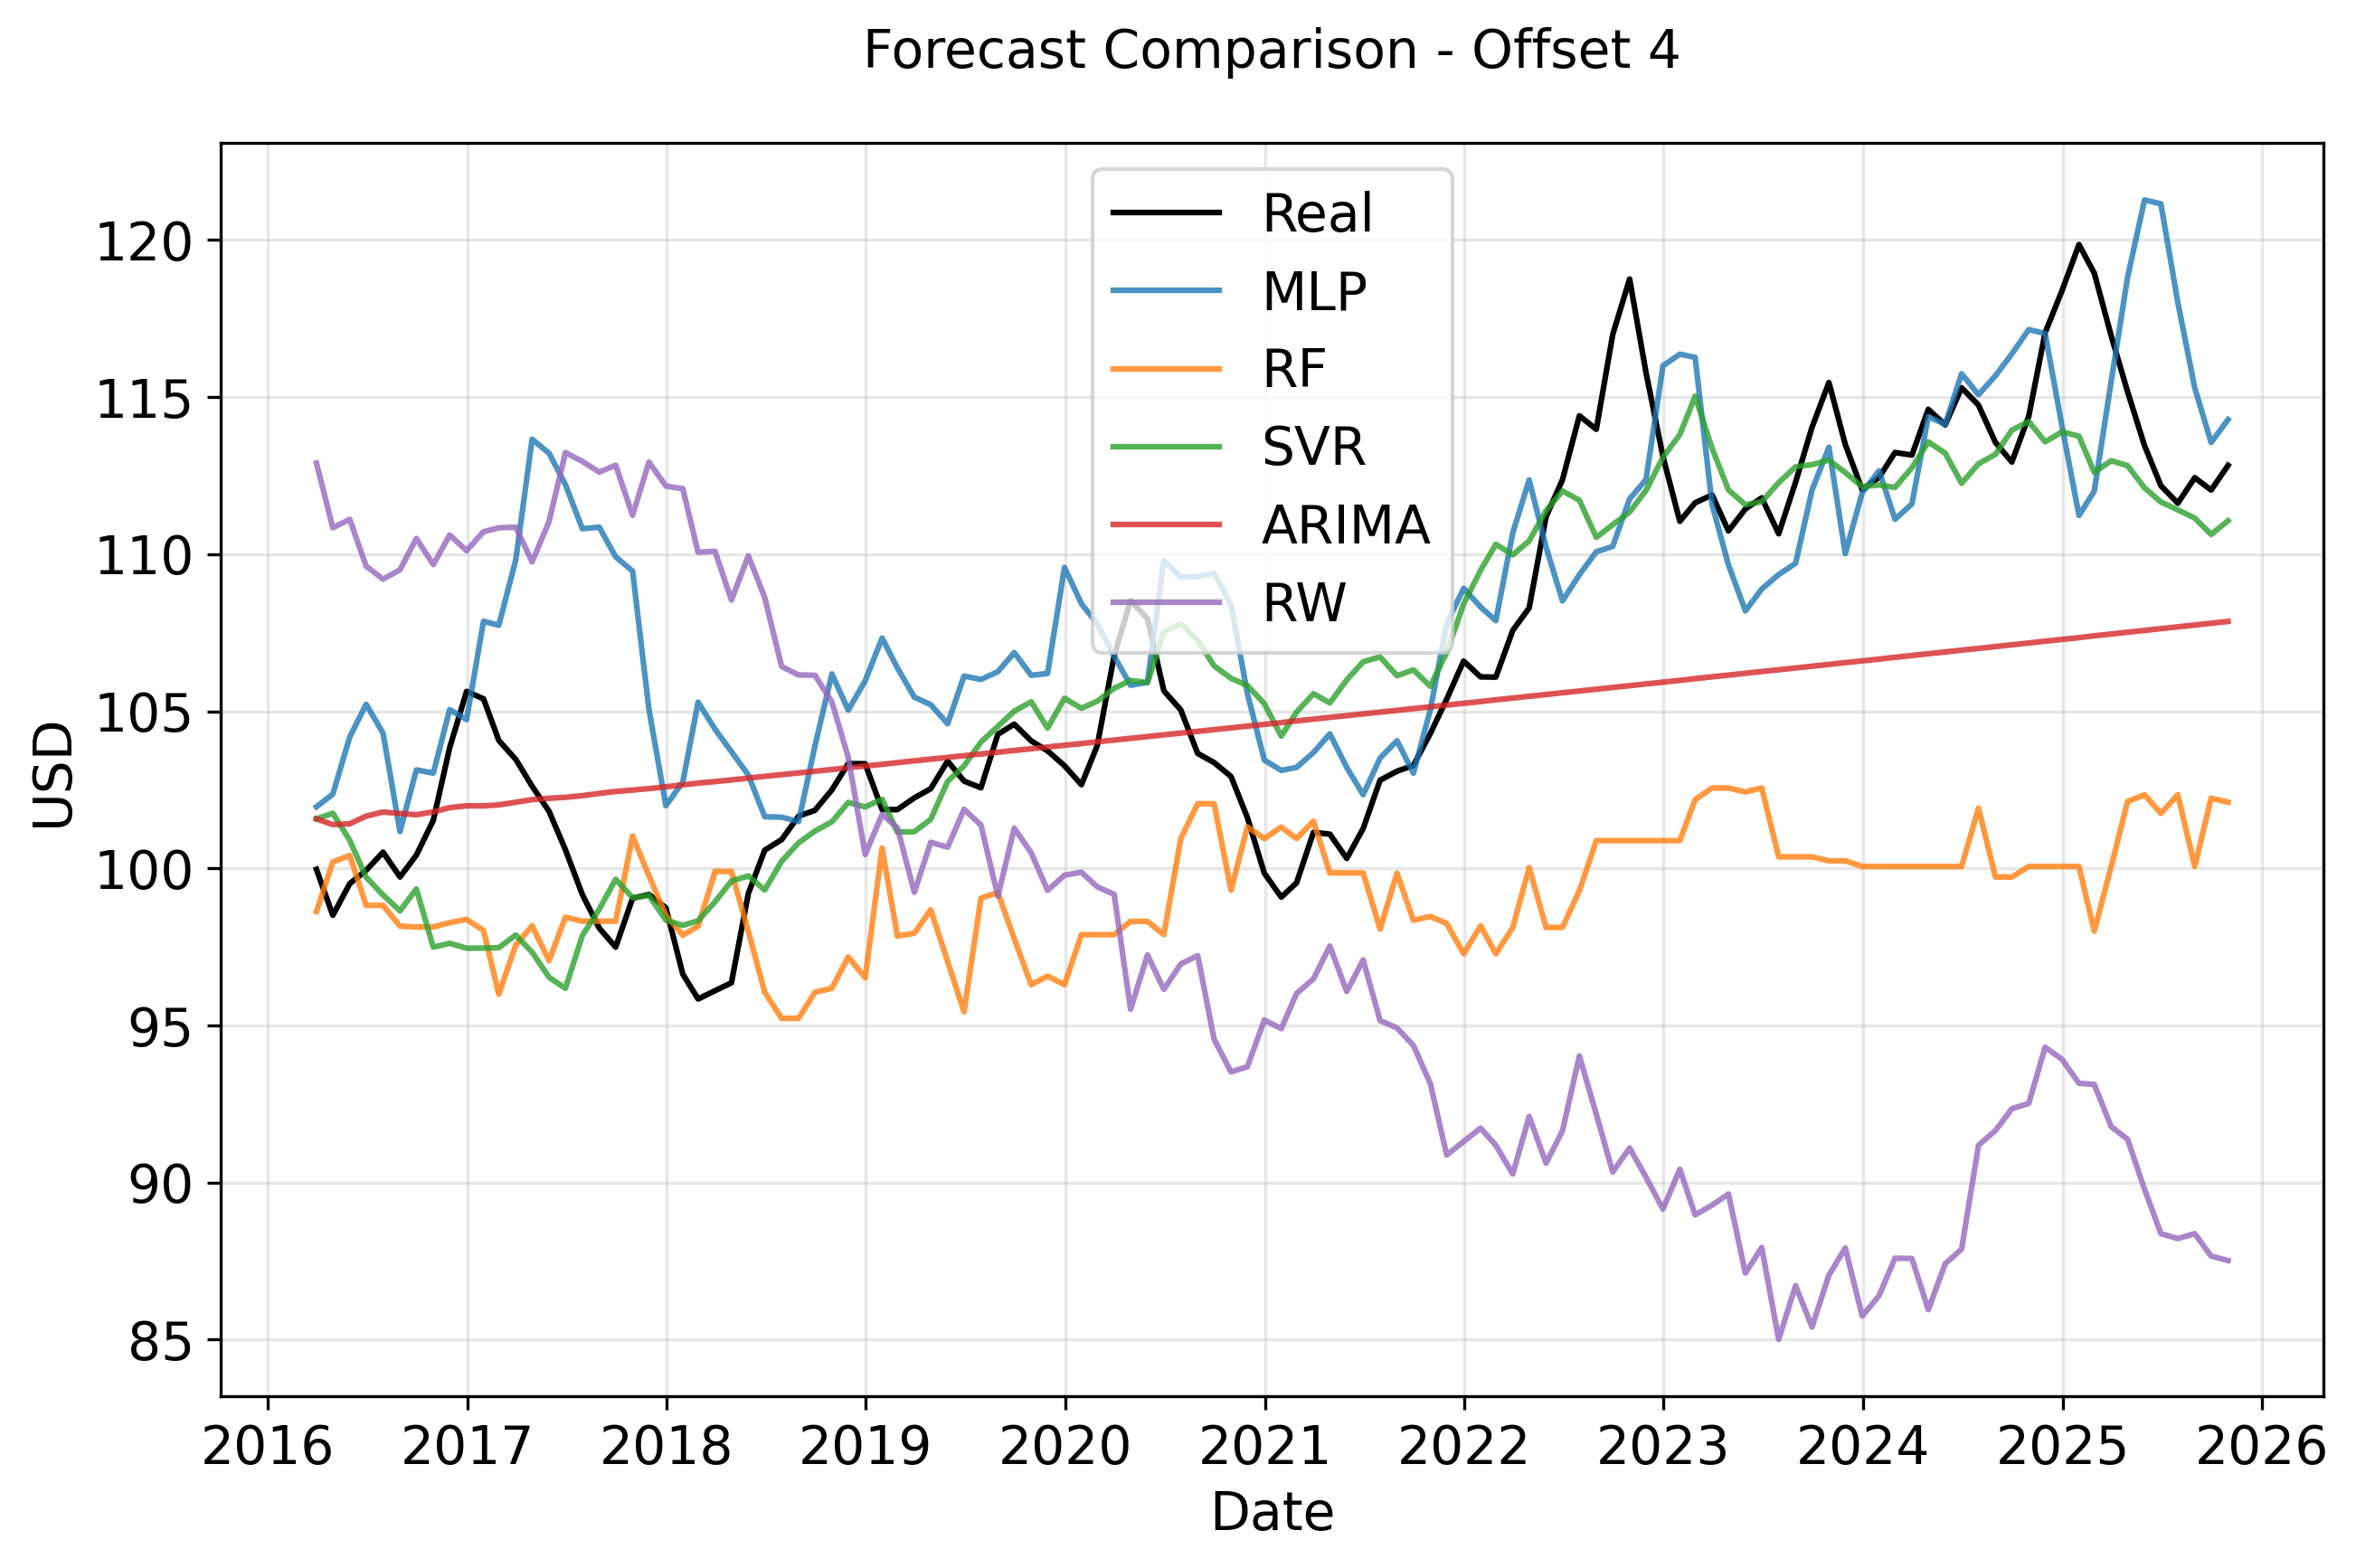
\includegraphics[width=\textwidth]{images/forecast-comparison/mse/4.png}
    \centering
    \caption{The best \gls{mse} forecasts per selected dataset per model for an offset of 4 months.}
    \label{fig:forecast-cmp-4}
\end{figure}

\begin{figure}[h]
    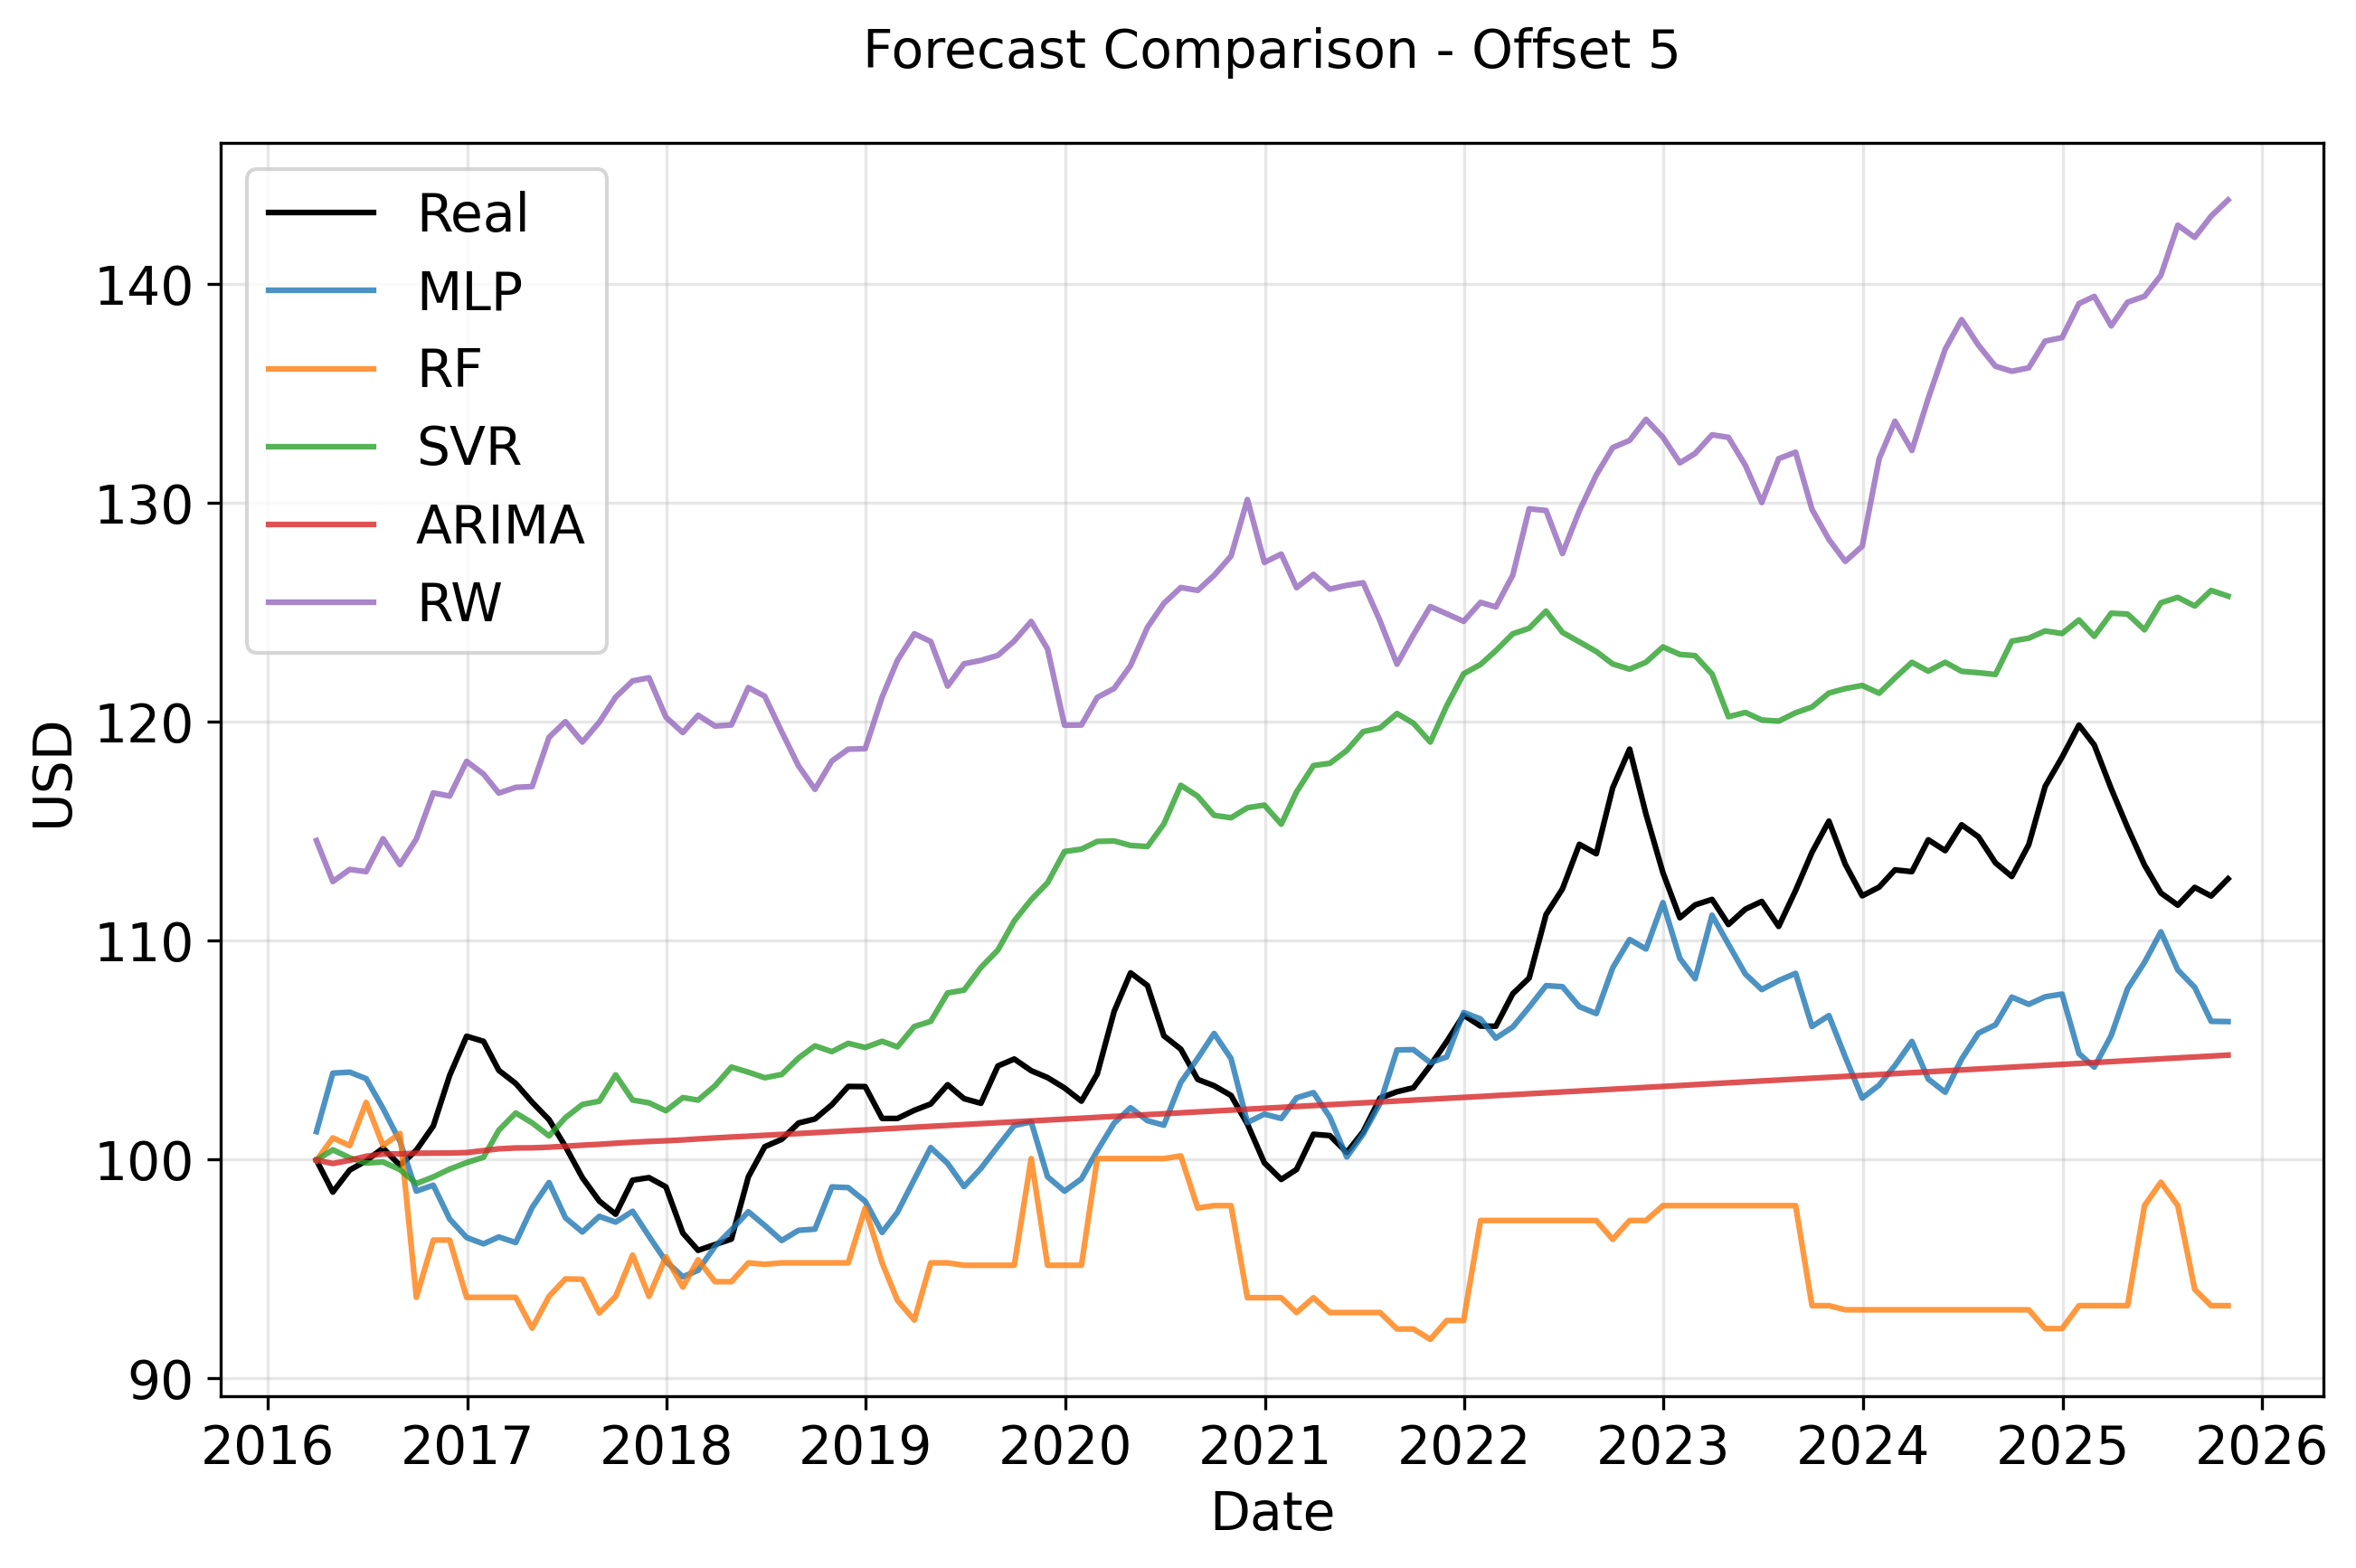
\includegraphics[width=\textwidth]{images/forecast-comparison/mse/5.png}
    \centering
    \caption{The best \gls{mse} forecasts per selected dataset per model for an offset of 5 months.}
    \label{fig:forecast-cmp-5}
\end{figure}

\begin{figure}[h]
    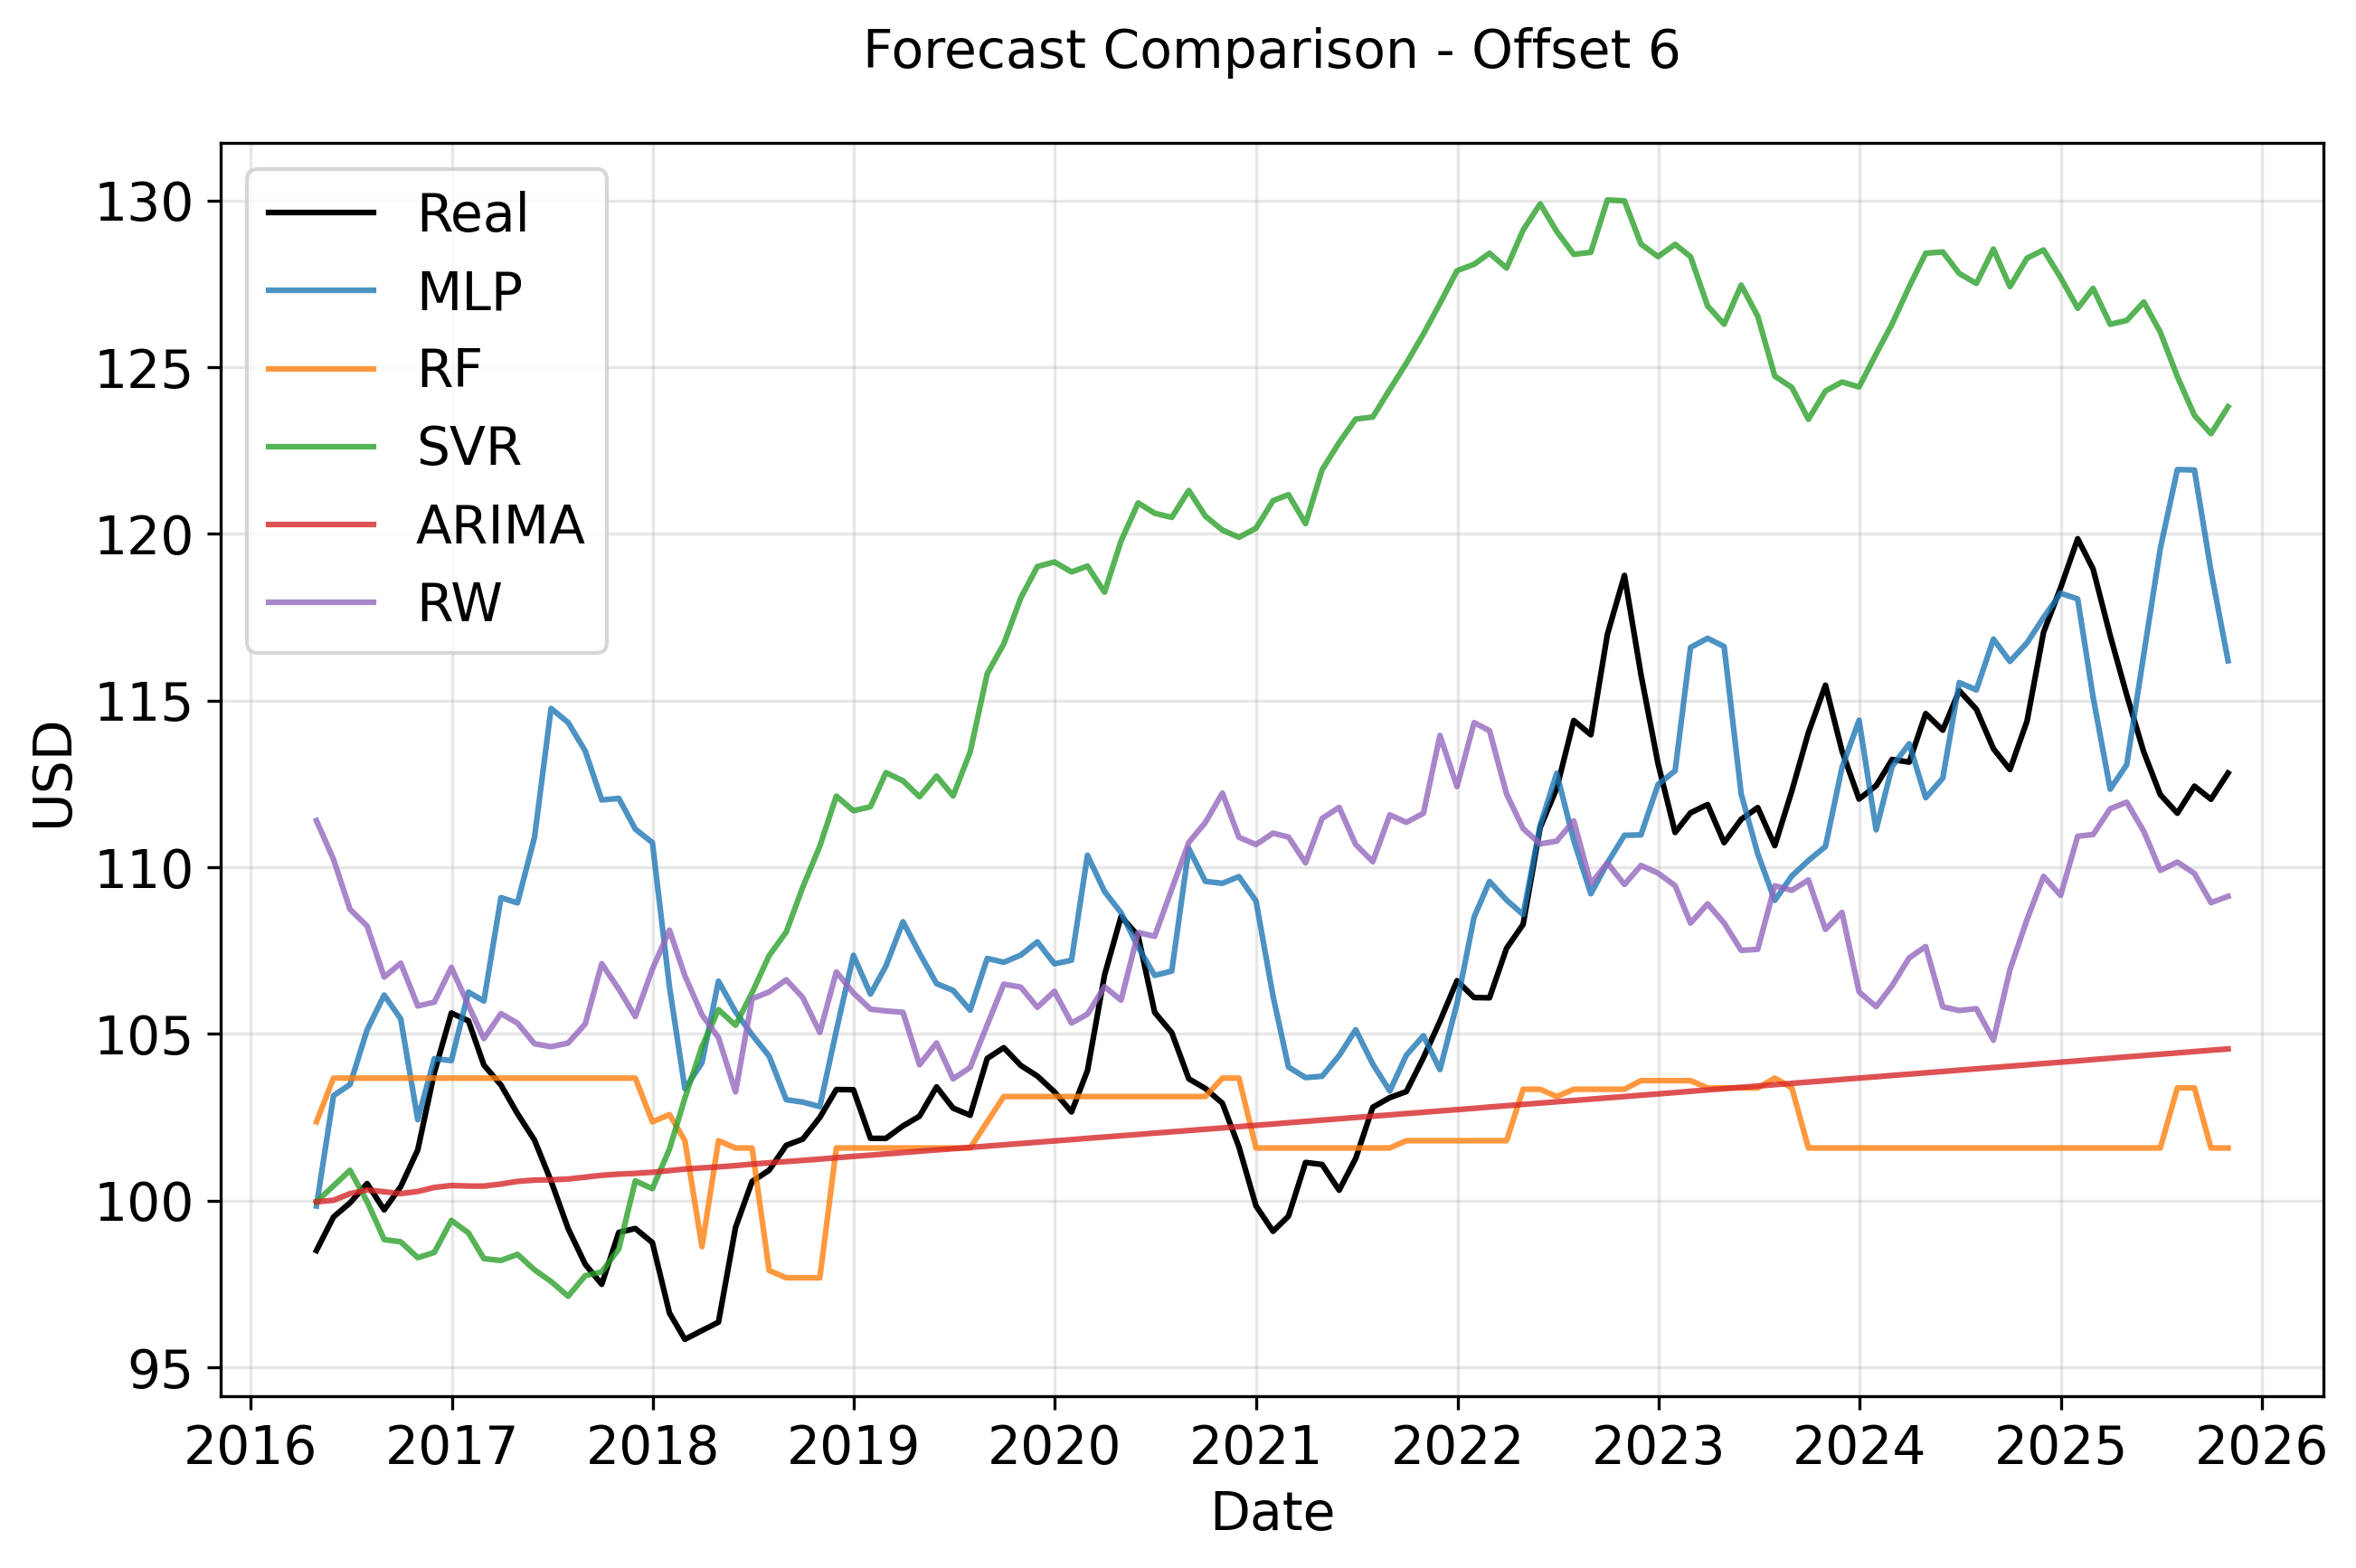
\includegraphics[width=\textwidth]{images/forecast-comparison/mse/6.png}
    \centering
    \caption{The best \gls{mse} forecasts per selected dataset per model for an offset of 6 months.}
    \label{fig:forecast-cmp-6}
\end{figure}

\begin{figure}[h]
    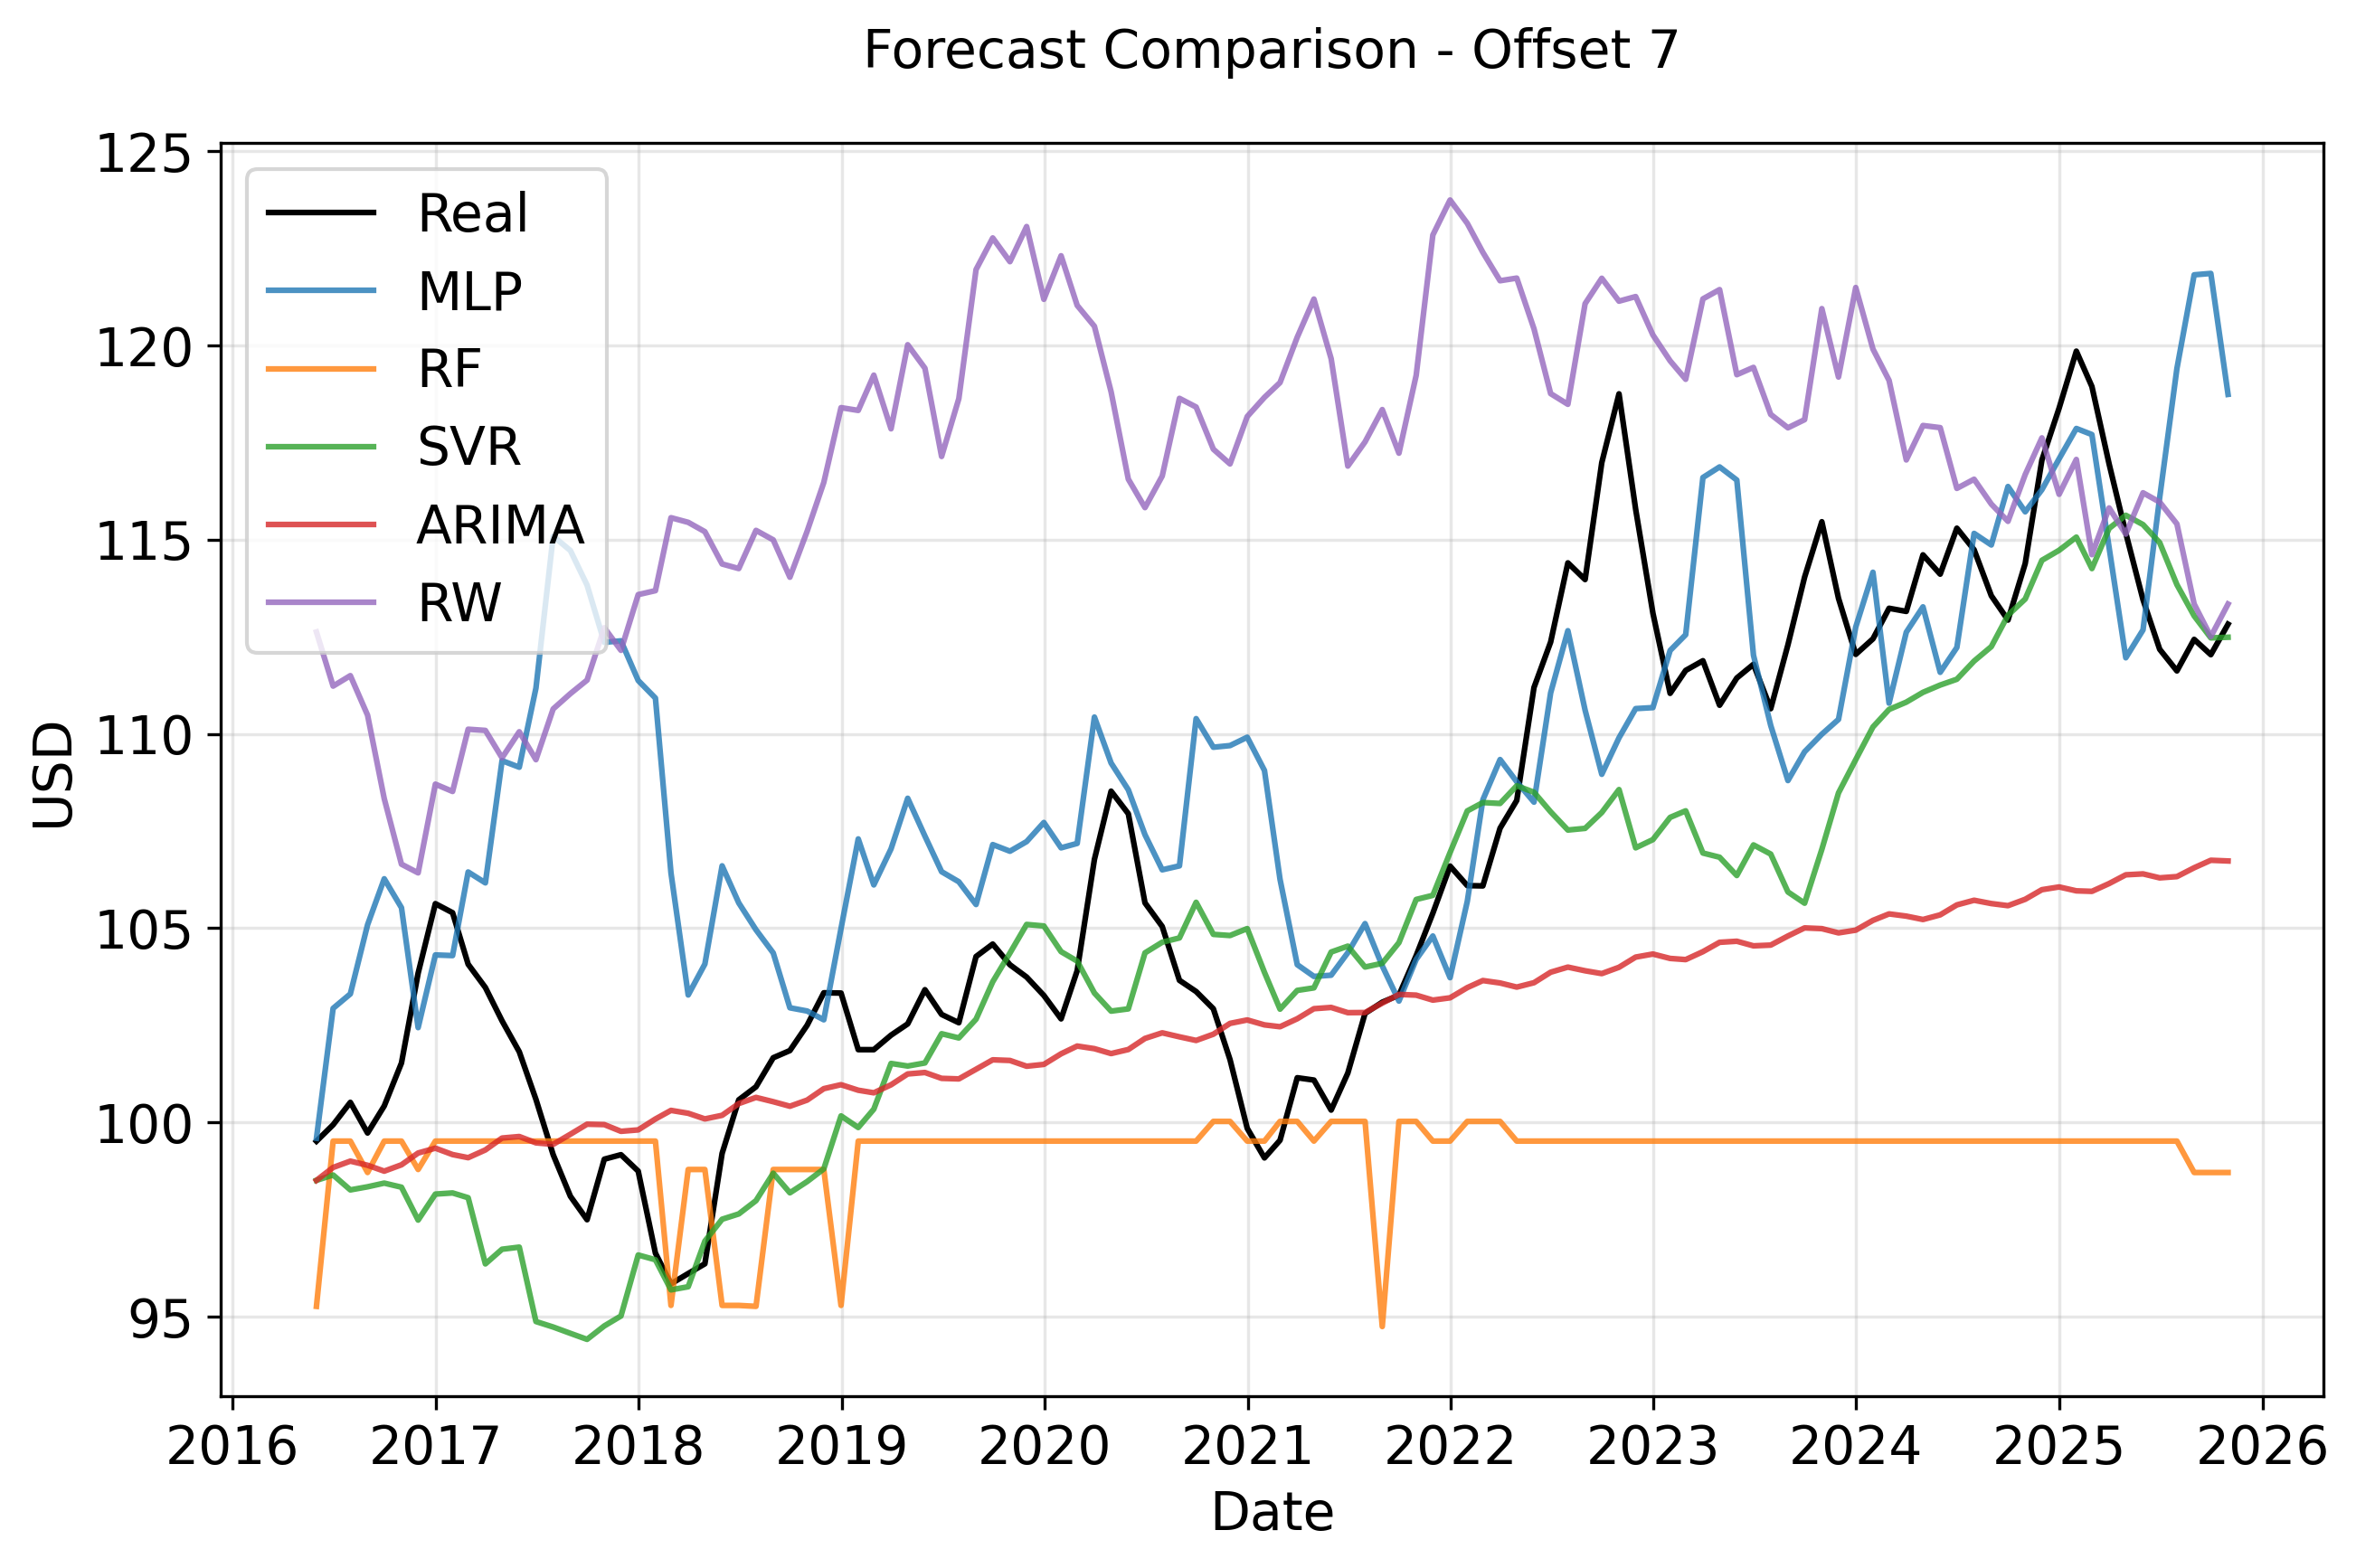
\includegraphics[width=\textwidth]{images/forecast-comparison/mse/7.png}
    \centering
    \caption{The best \gls{mse} forecasts per selected dataset per model for an offset of 7 months.}
    \label{fig:forecast-cmp-7}
\end{figure}

\begin{figure}[h]
    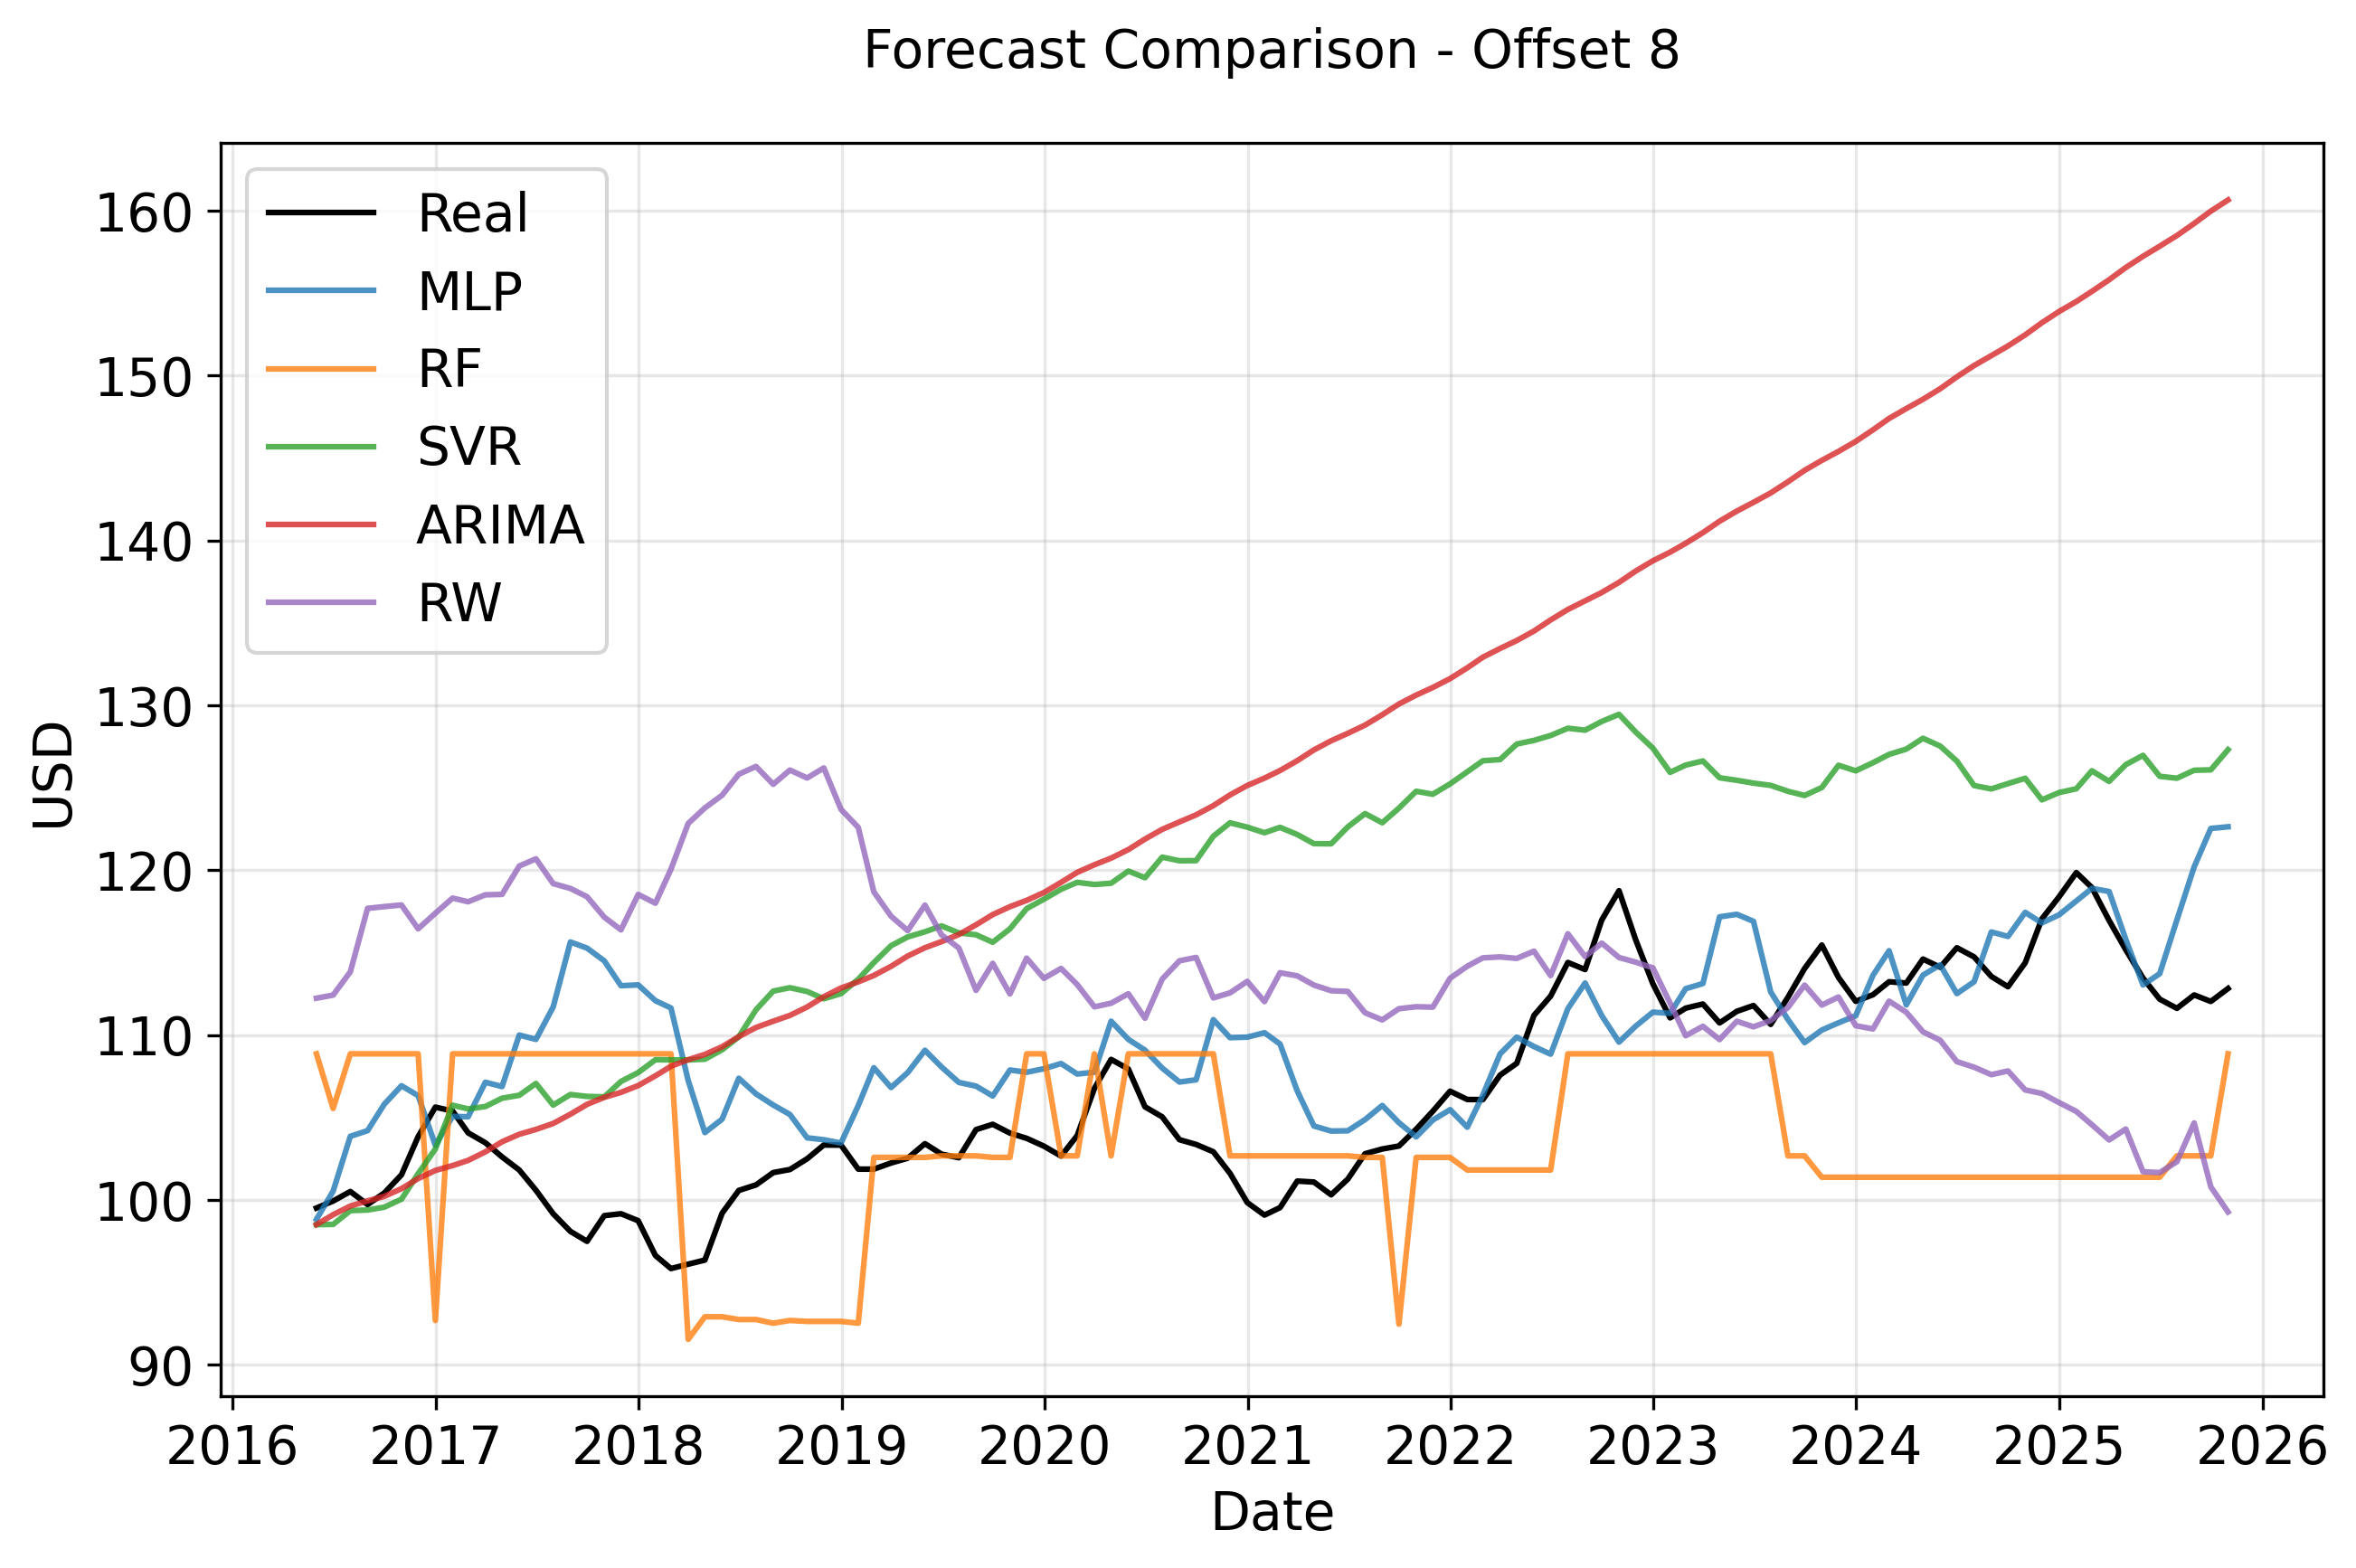
\includegraphics[width=\textwidth]{images/forecast-comparison/mse/8.png}
    \centering
    \caption{The best \gls{mse} forecasts per selected dataset per model for an offset of 8 months.}
    \label{fig:forecast-cmp-8}
\end{figure}

\begin{figure}[h]
    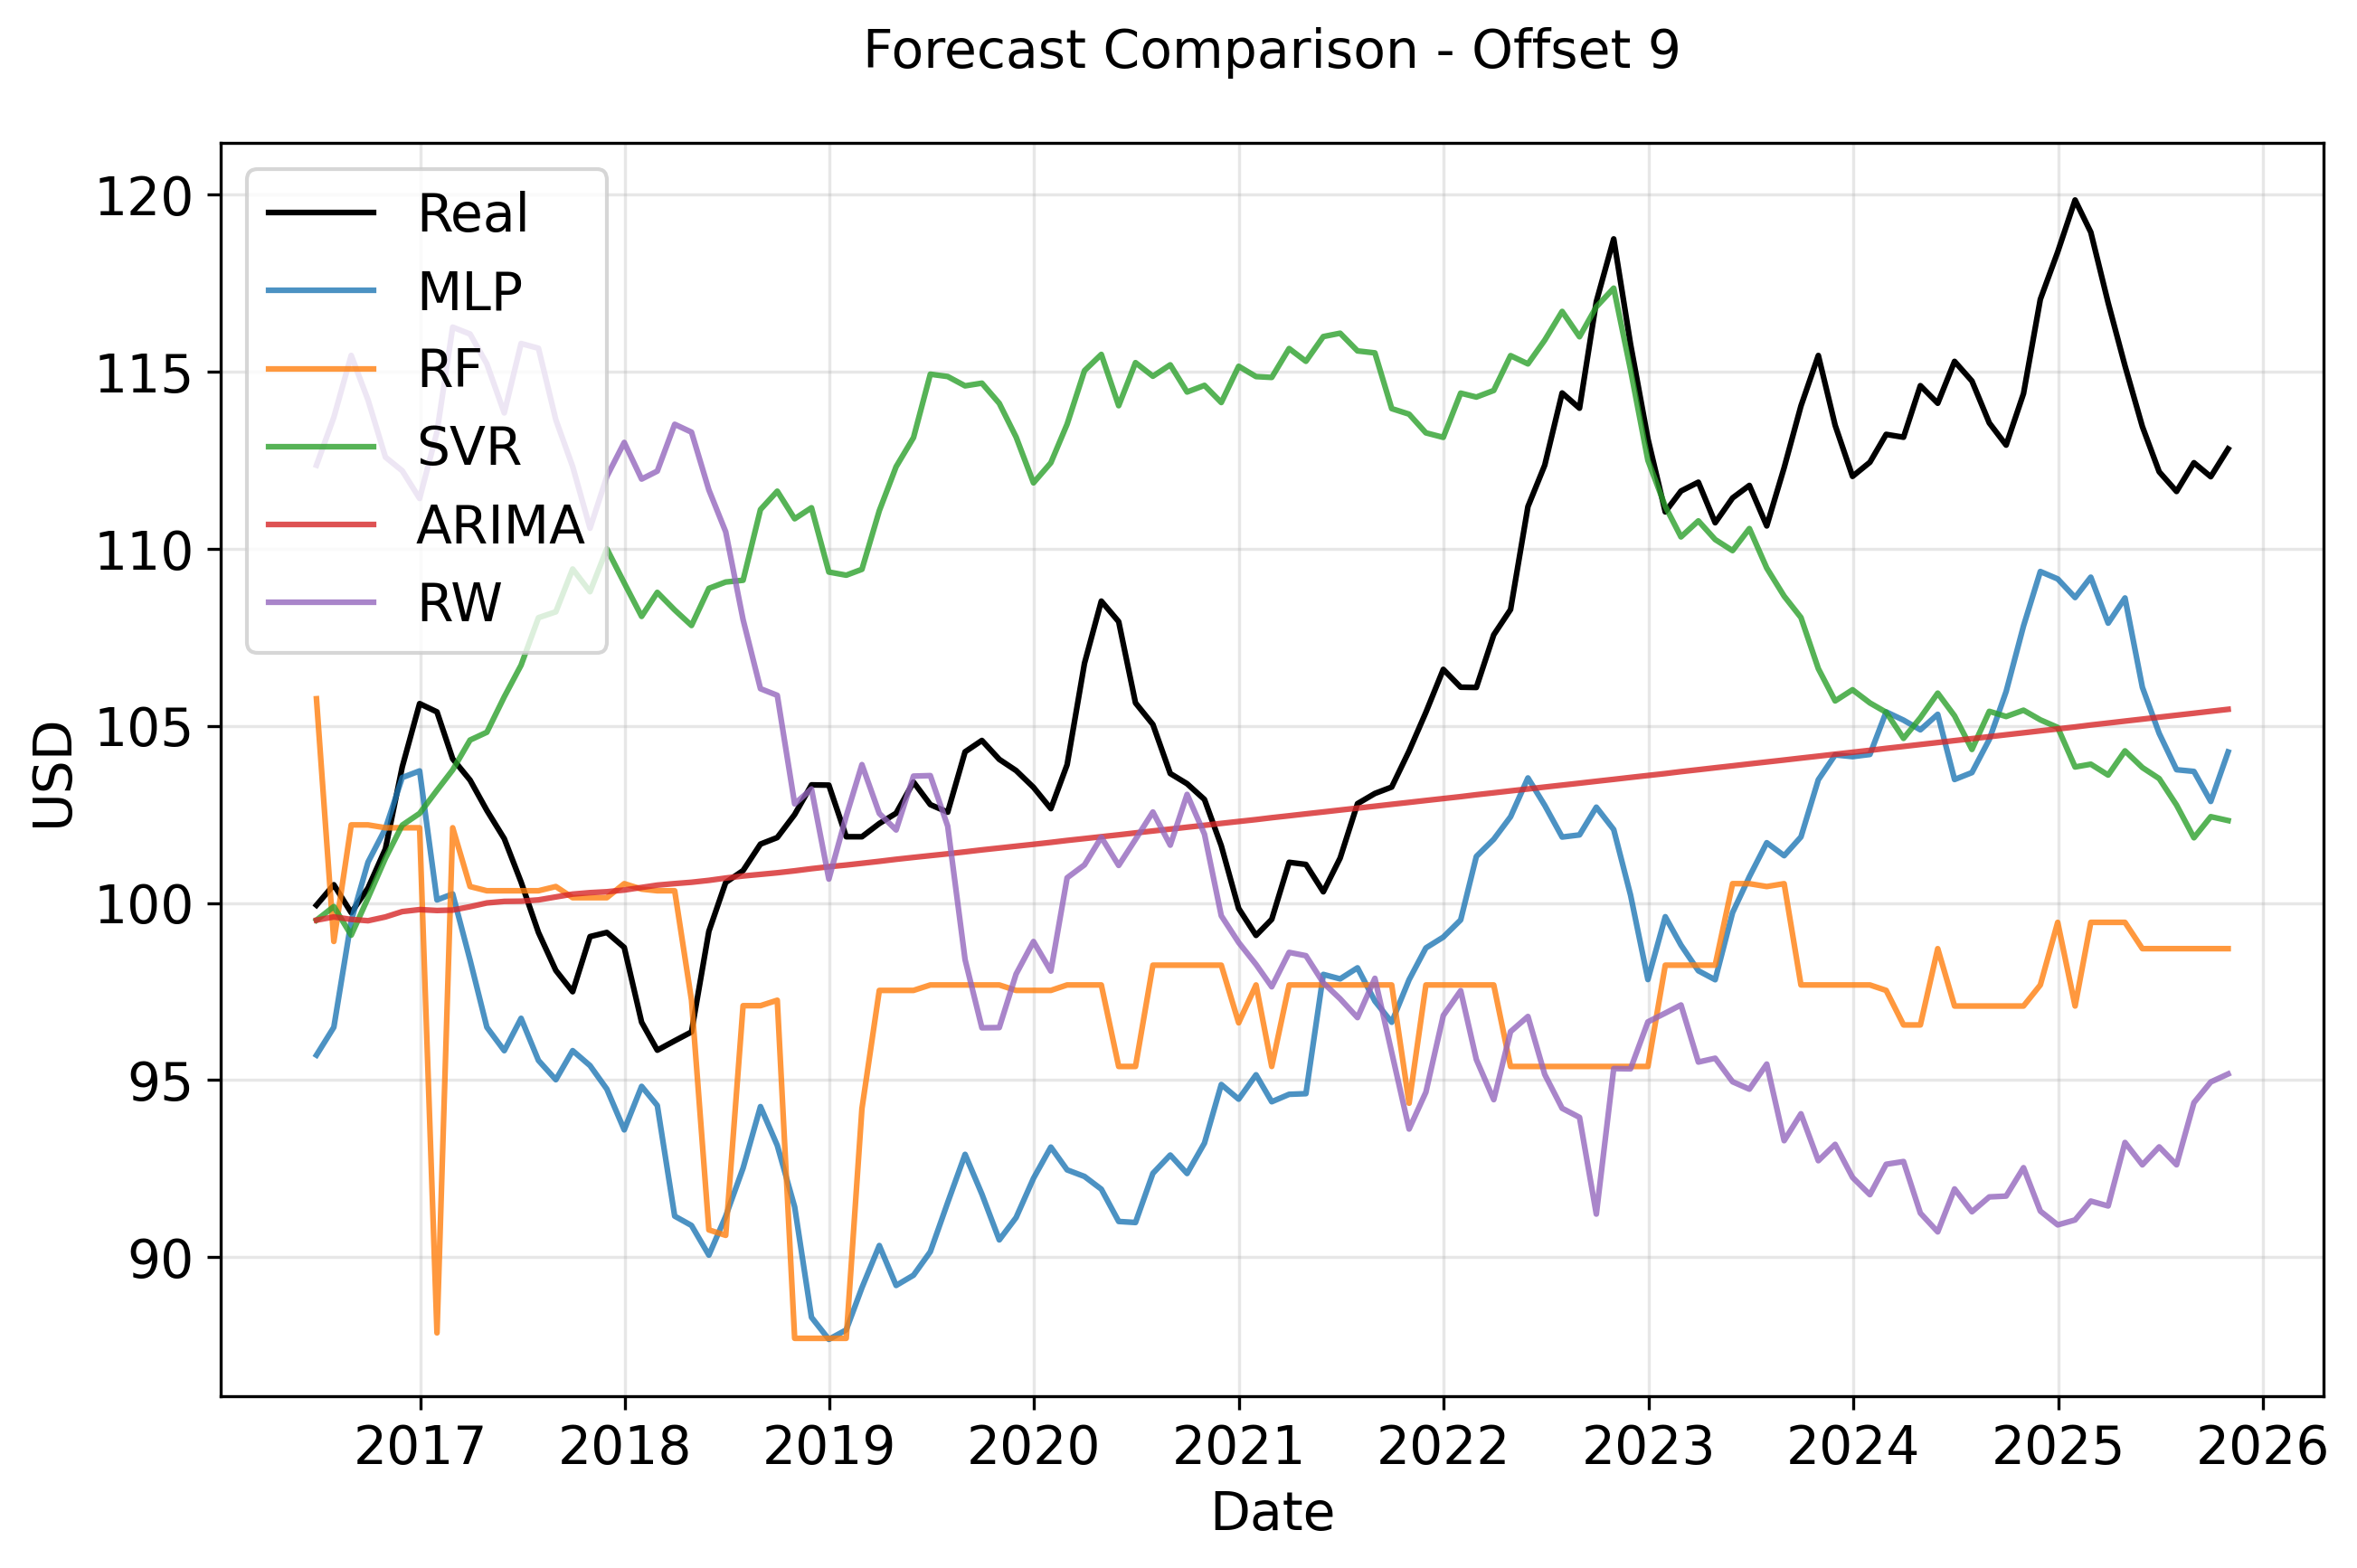
\includegraphics[width=\textwidth]{images/forecast-comparison/mse/9.png}
    \centering
    \caption{The best \gls{mse} forecasts per selected dataset per model for an offset of 9 months.}
    \label{fig:forecast-cmp-9}
\end{figure}

\begin{figure}[h]
    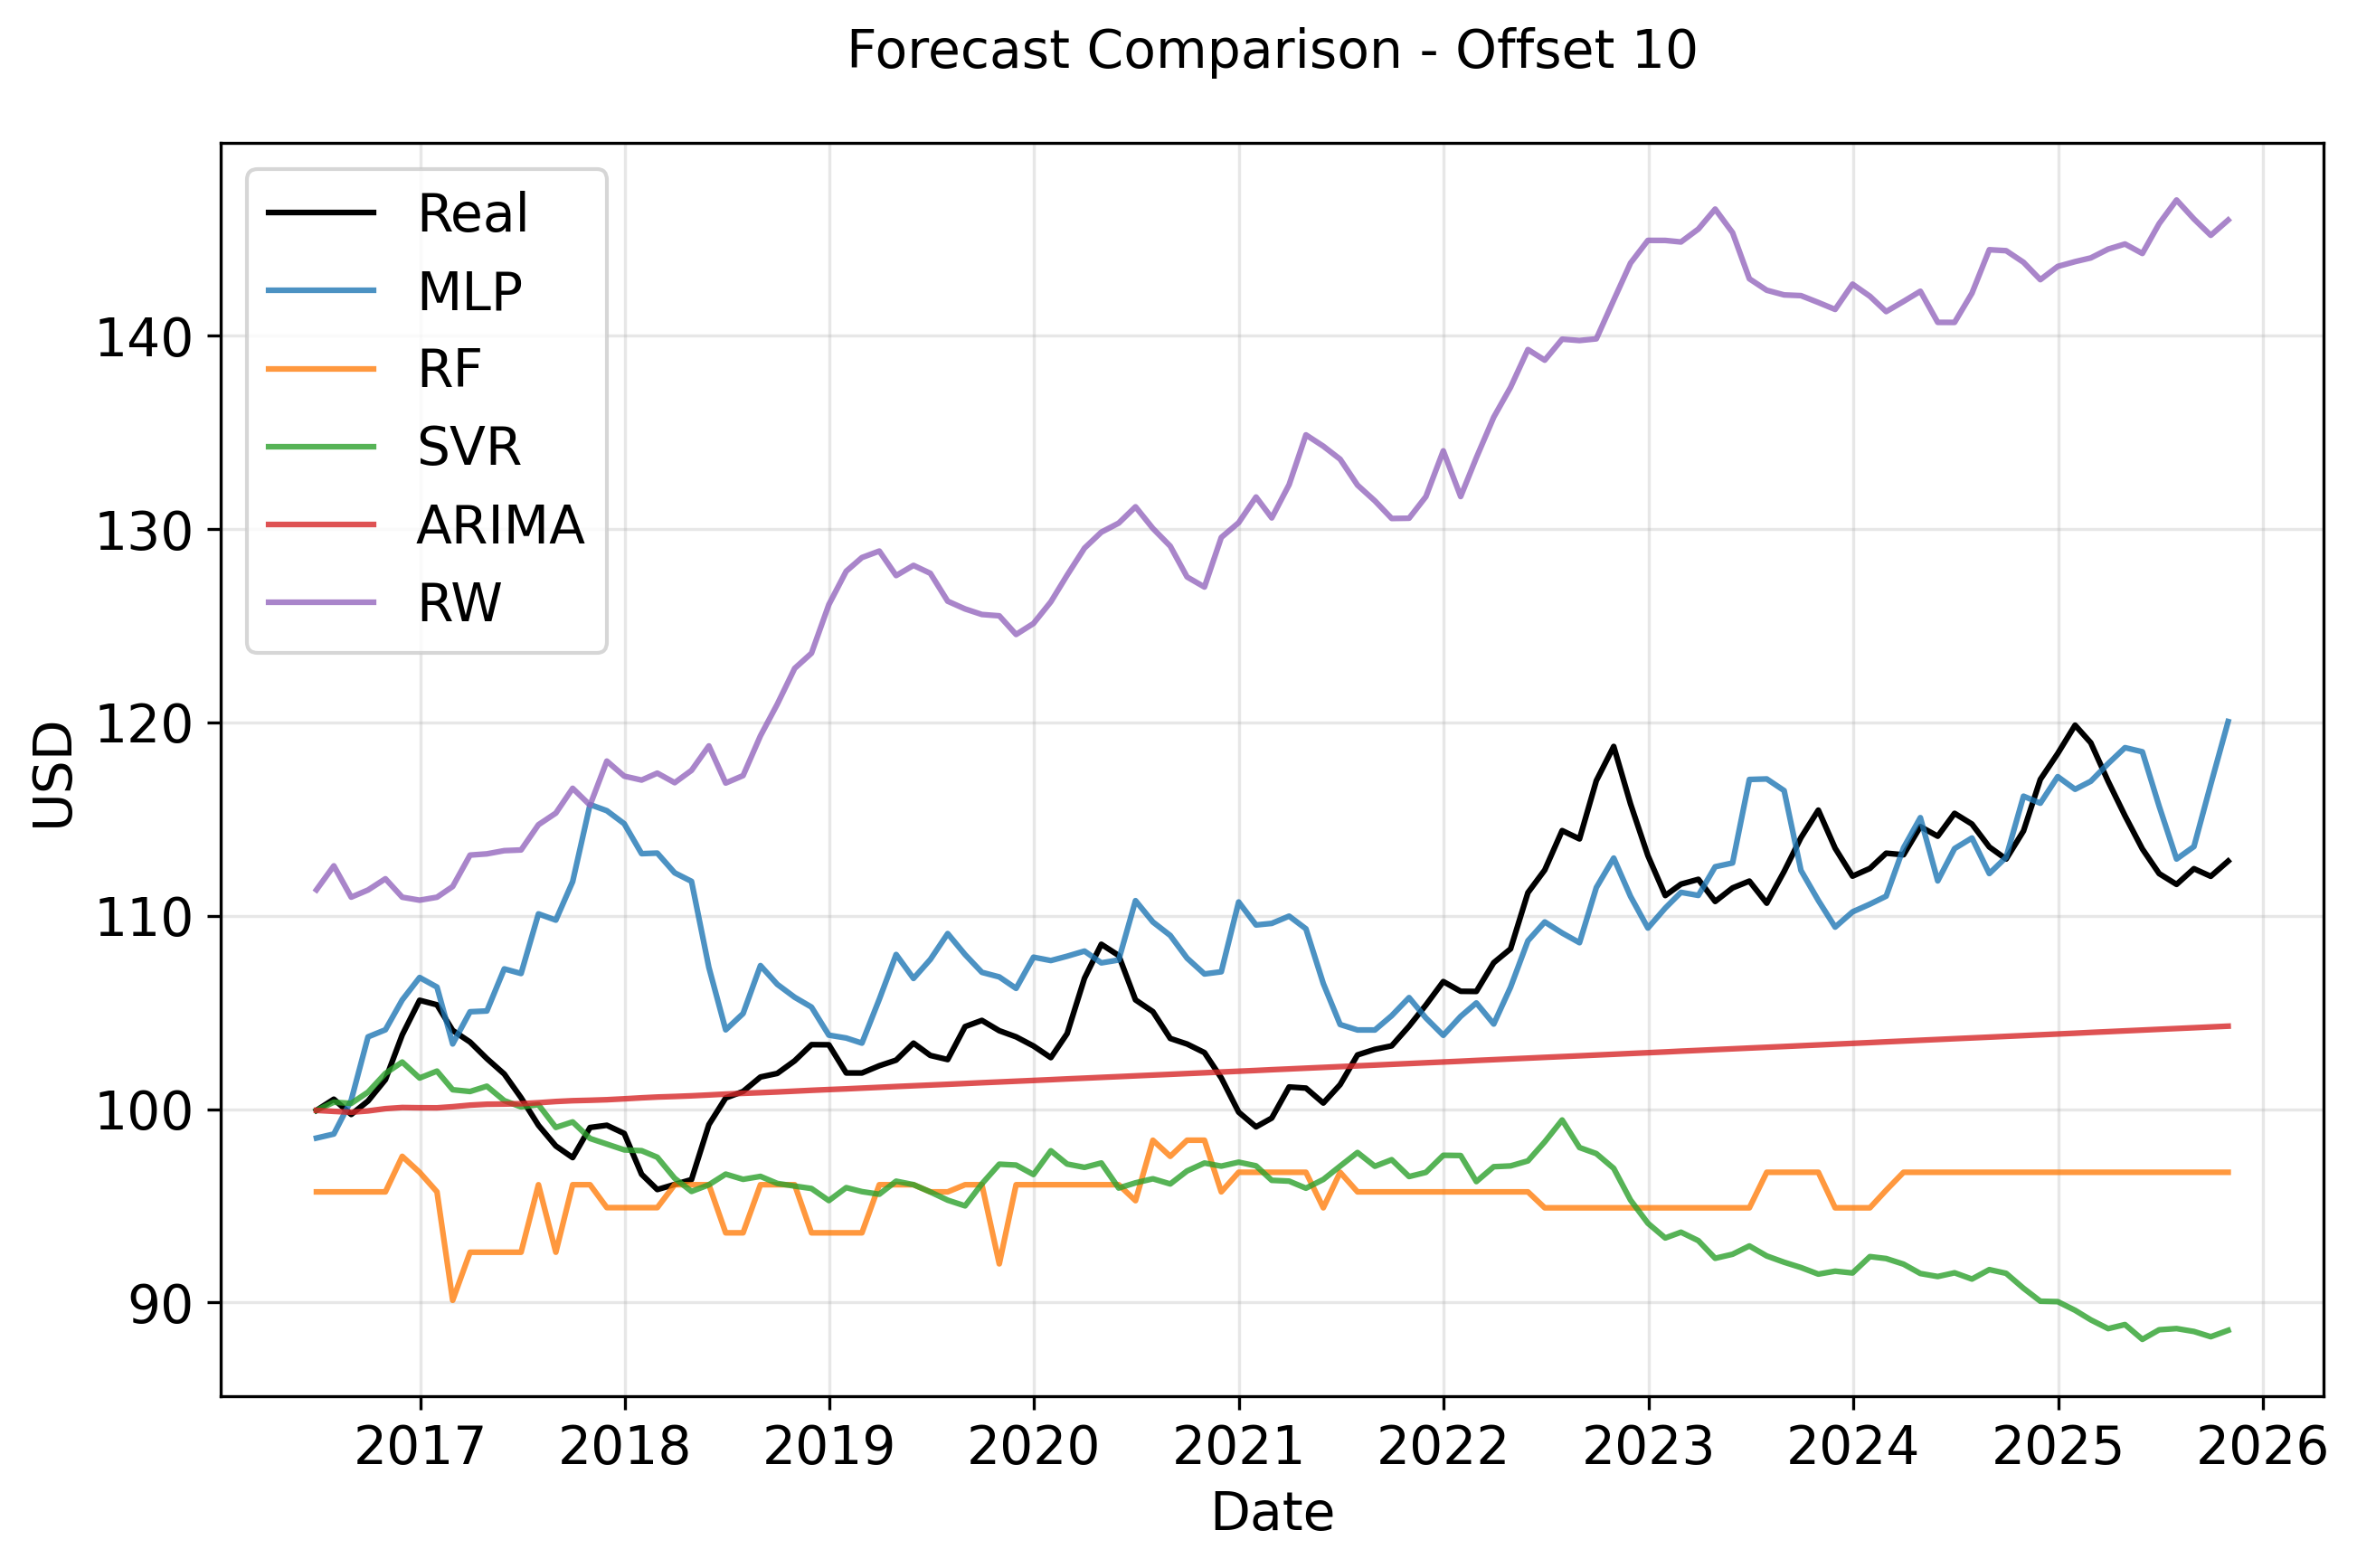
\includegraphics[width=\textwidth]{images/forecast-comparison/mse/10.png}
    \centering
    \caption{The best \gls{mse} forecasts per selected dataset per model for an offset of 10 months.}
    \label{fig:forecast-cmp-10}
\end{figure}

\begin{figure}[h]
    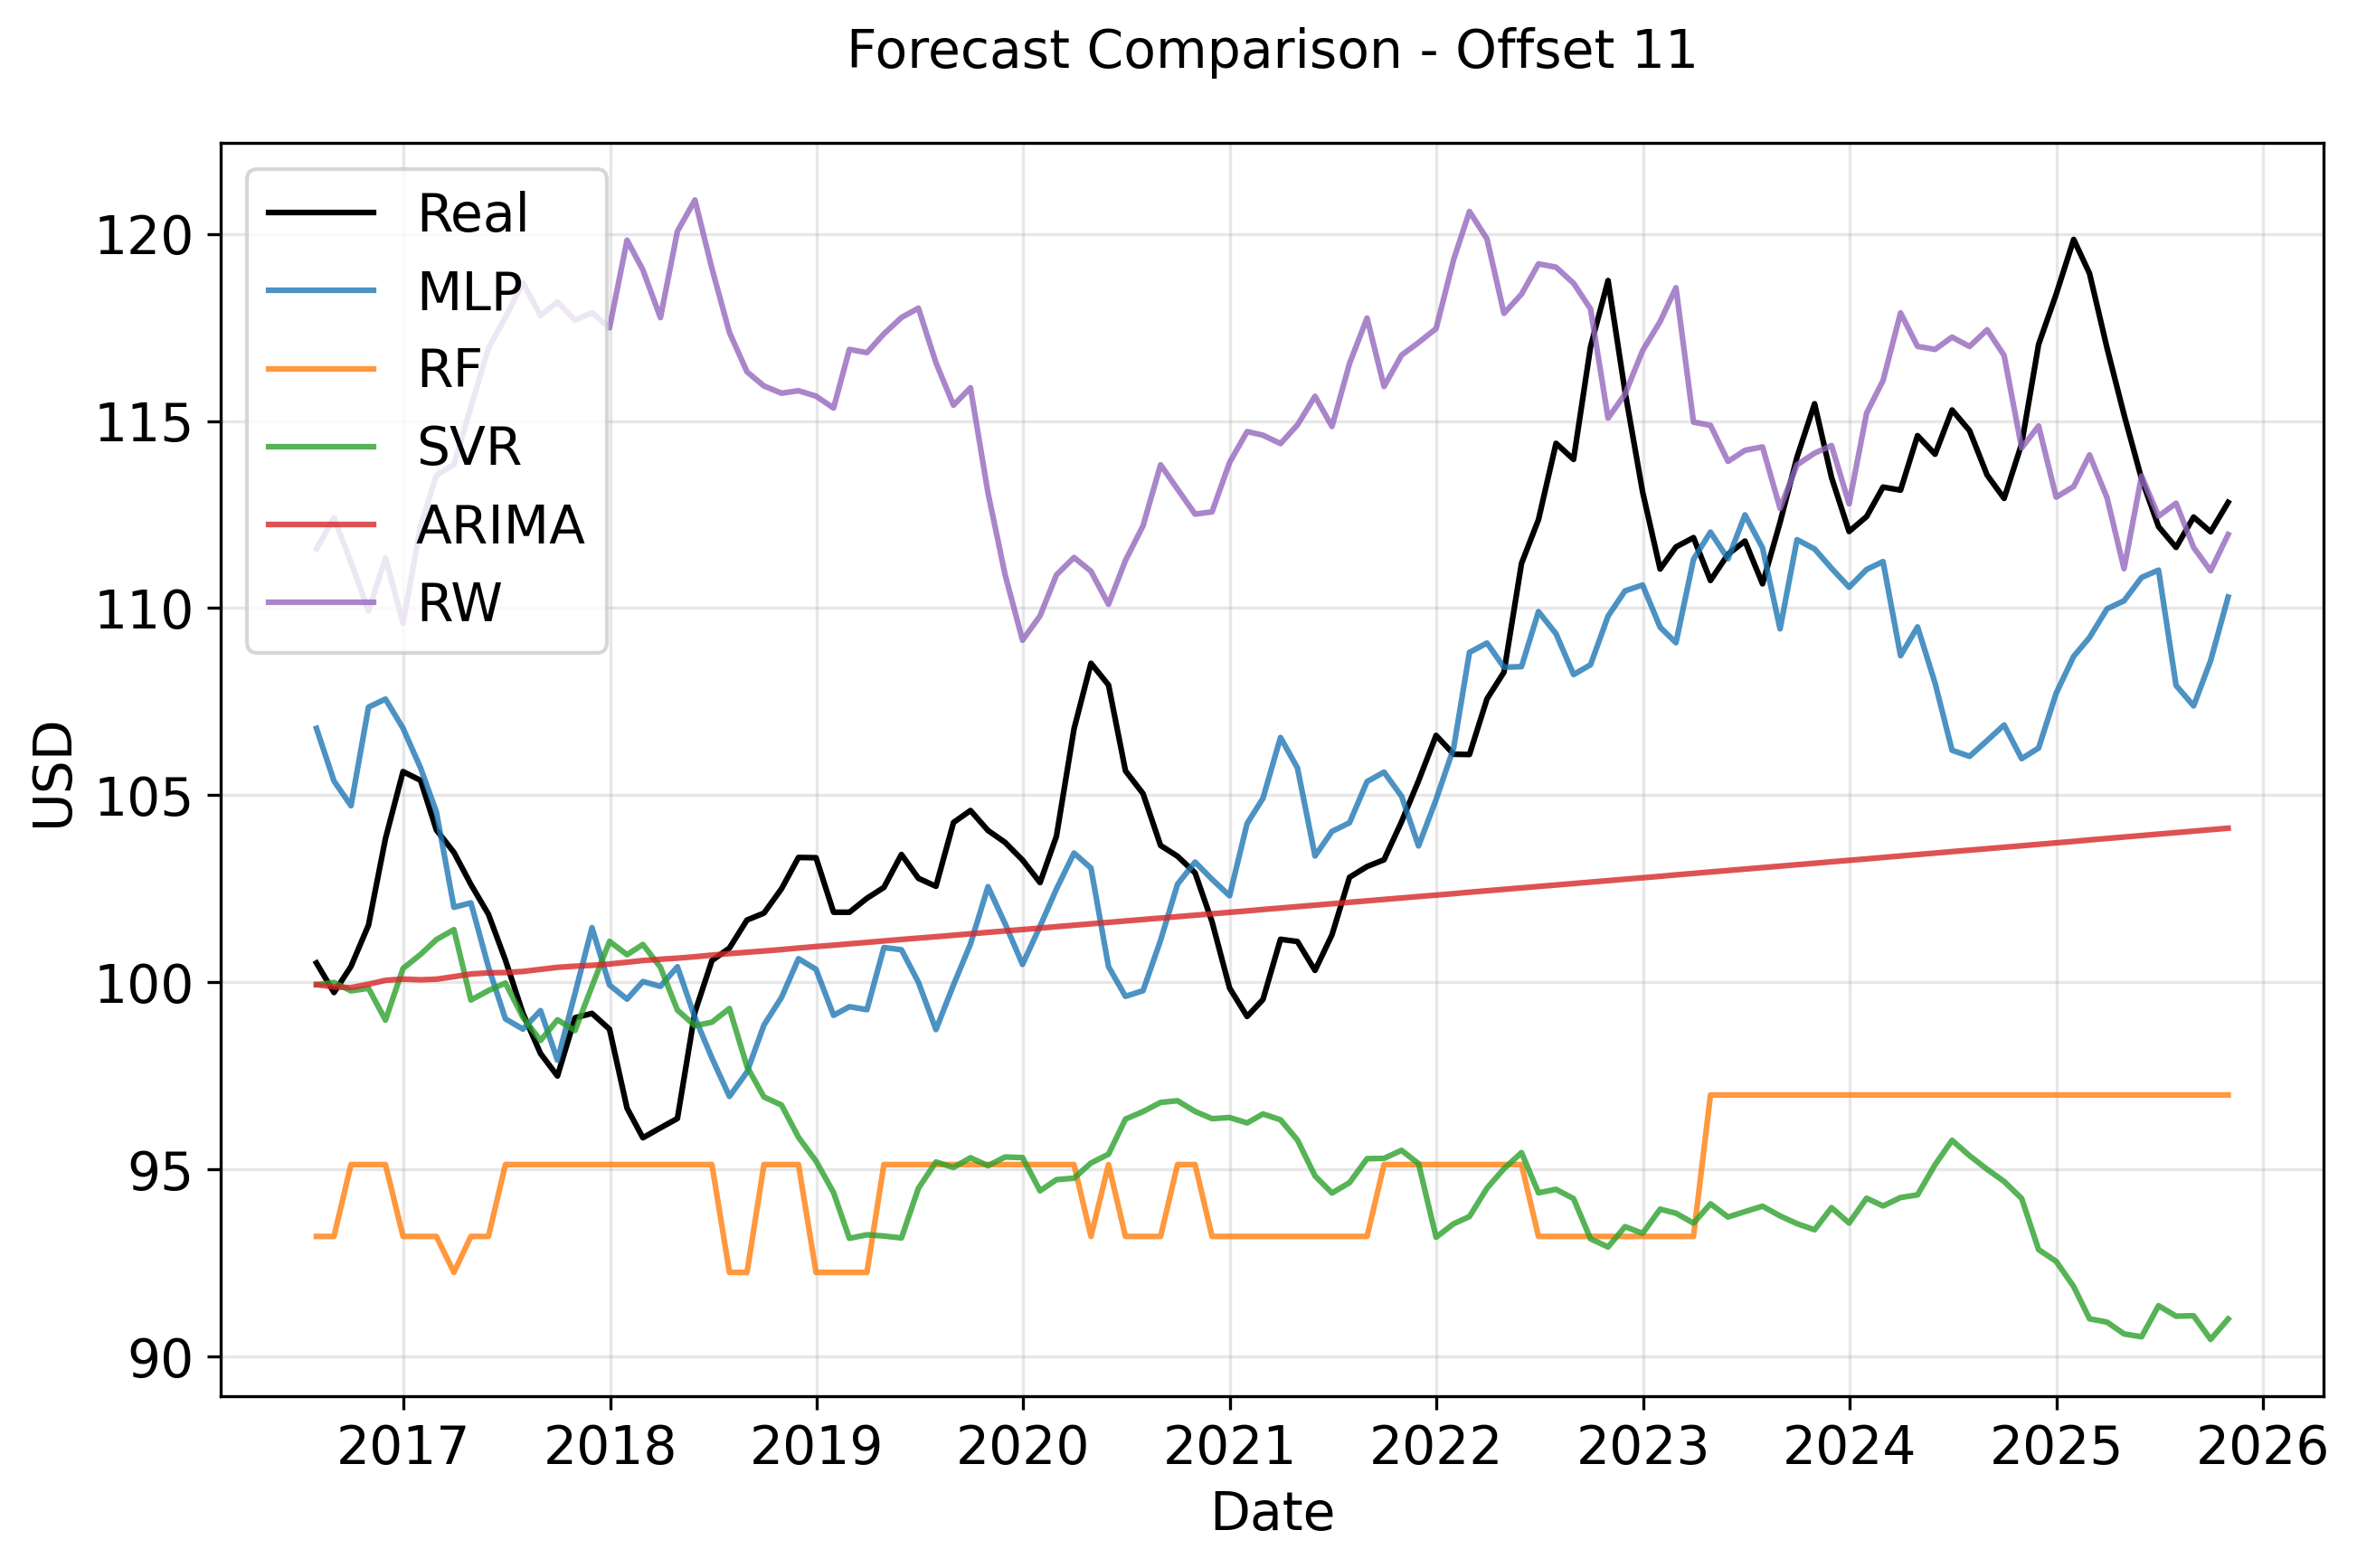
\includegraphics[width=\textwidth]{images/forecast-comparison/mse/11.png}
    \centering
    \caption{The best \gls{mse} forecasts per selected dataset per model for an offset of 11 months.}
    \label{fig:forecast-cmp-11}
\end{figure}

\begin{figure}[h]
    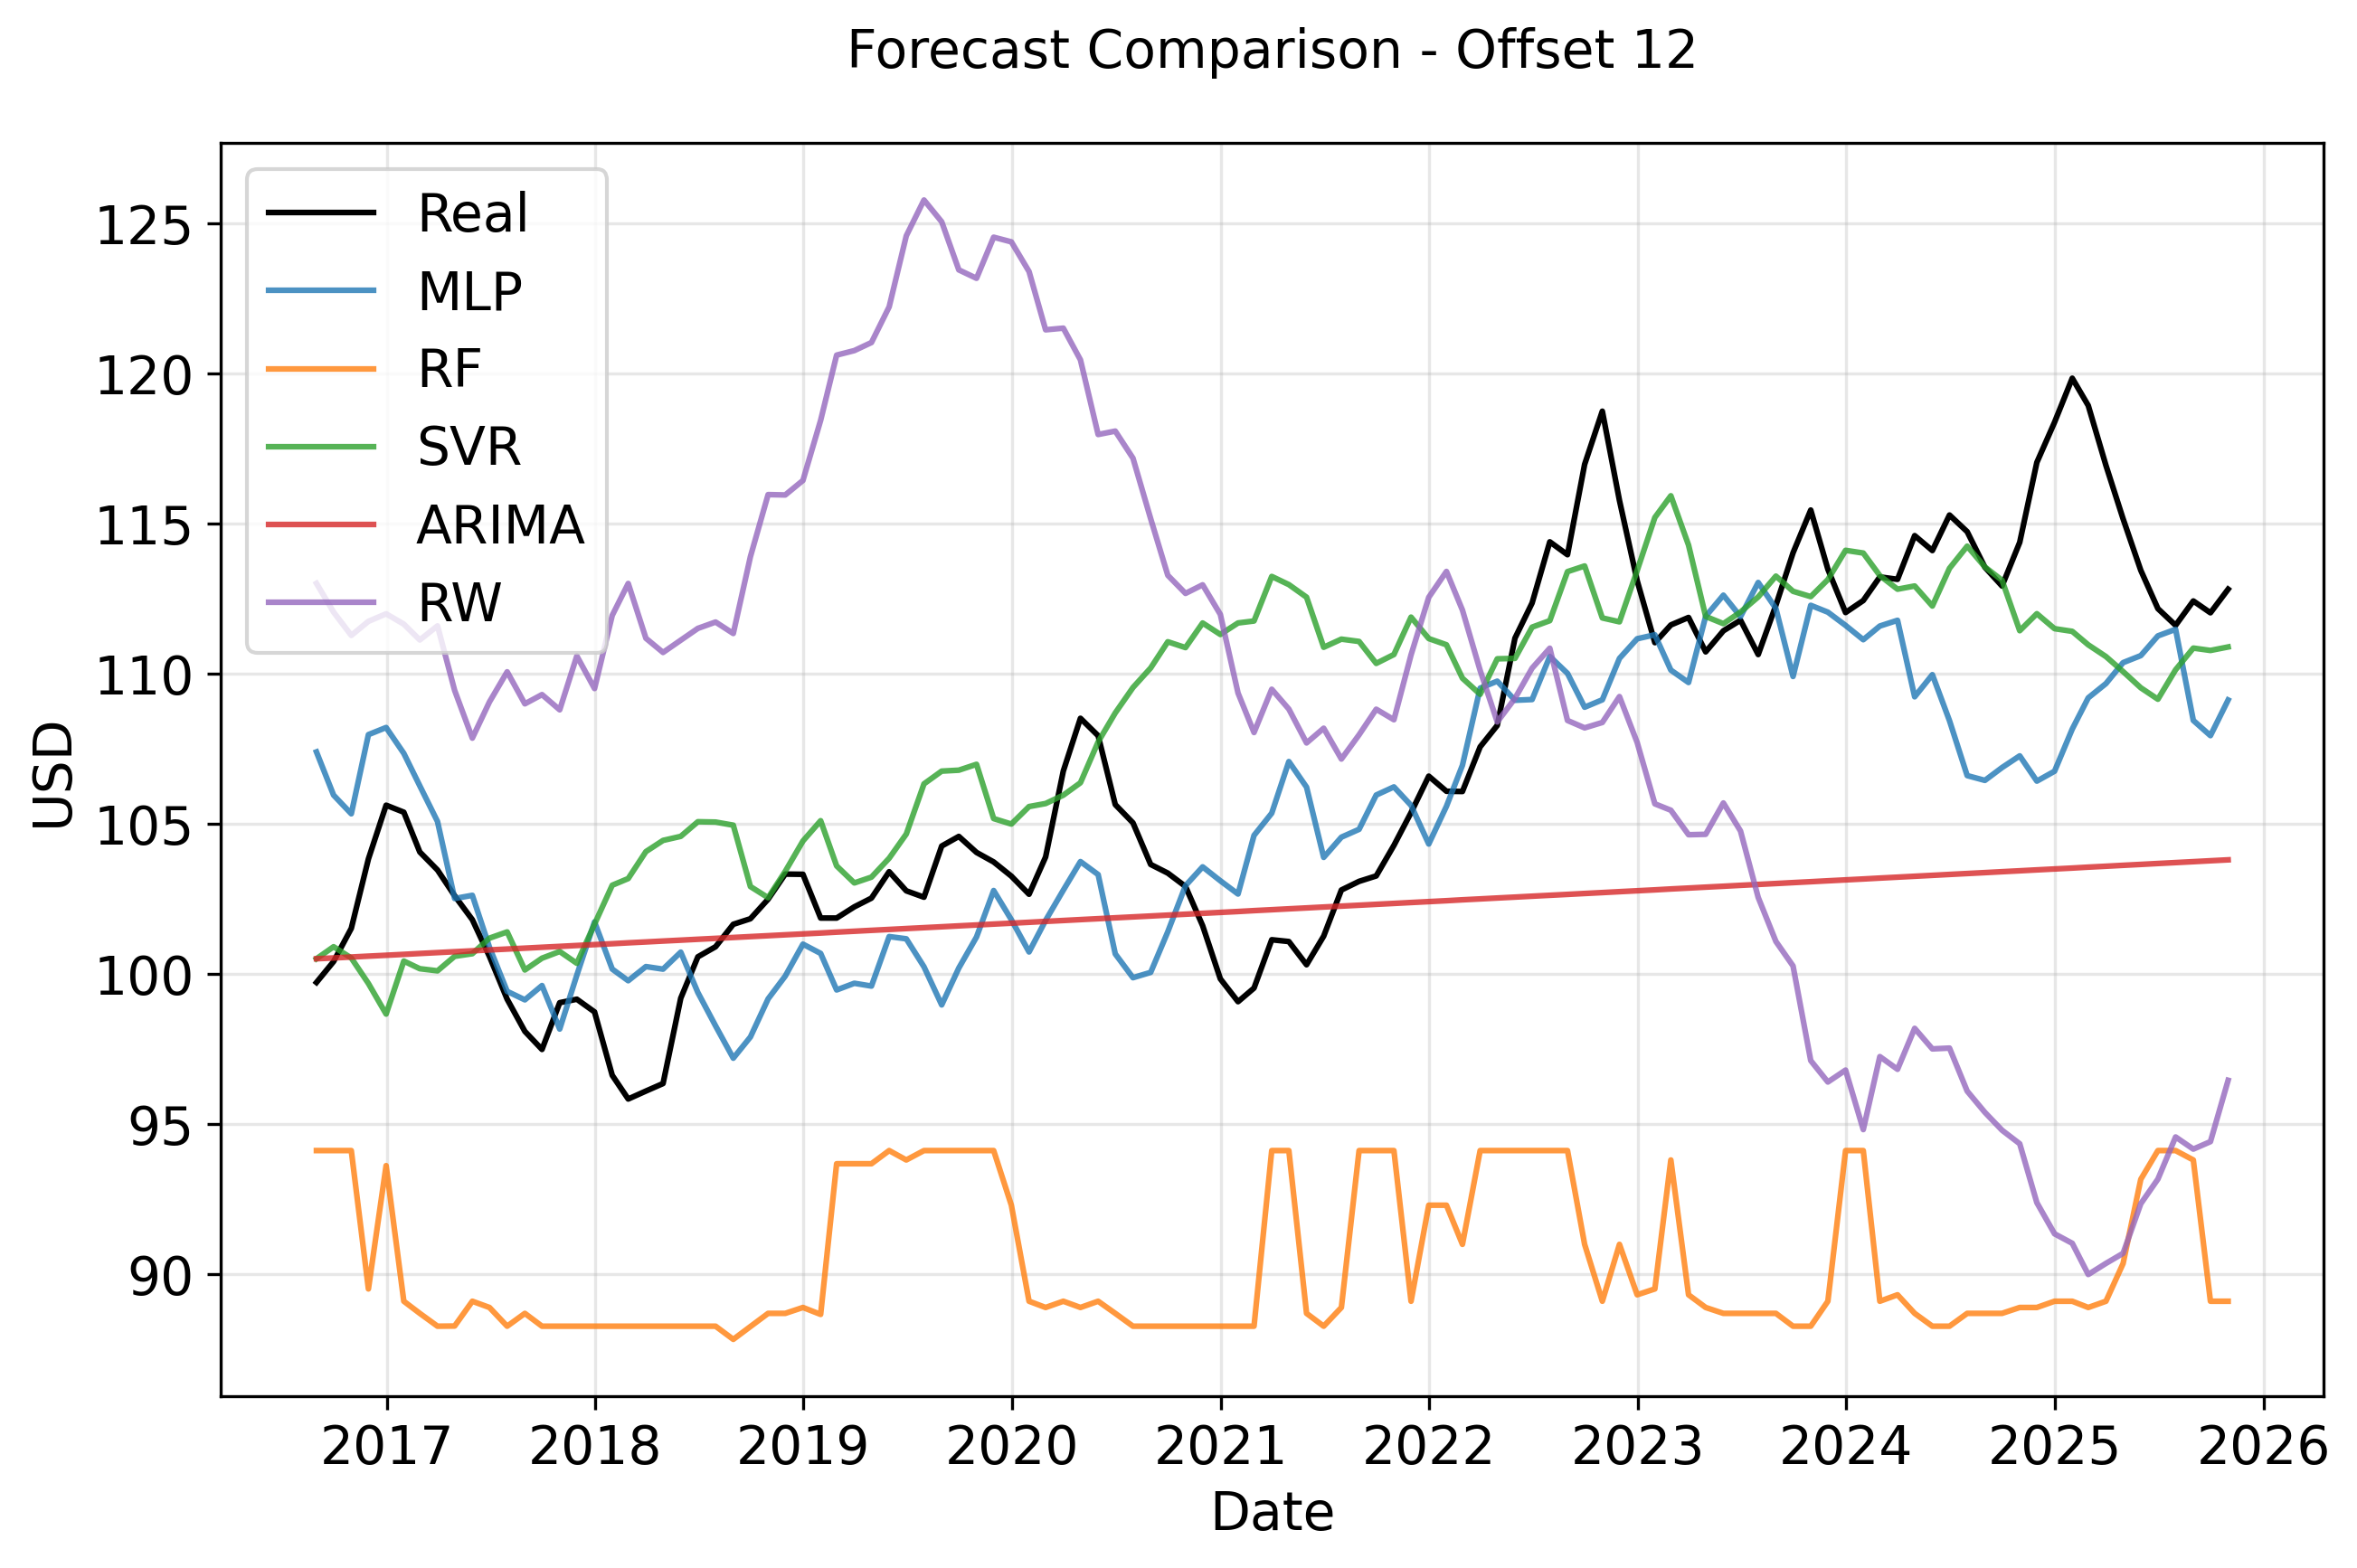
\includegraphics[width=\textwidth]{images/forecast-comparison/mse/12.png}
    \centering
    \caption{The best \gls{mse} forecasts per selected dataset per model for an offset of 12 months.}
    \label{fig:forecast-cmp-12}
\end{figure}

